\documentclass[12pt,b5paper,landscape]{article}
\usepackage{multicol}
%\setlength\paperwidth{297mm}
%\setlength\paperheight{210mm}
\usepackage[CJKnumber,fallback]{xeCJK}
\setCJKmainfont[BoldFont={Adobe Heiti Std},ItalicFont={Adobe Kaiti Std}]{Adobe Song Std}
\setCJKfamilyfont{vert}[RawFeature={vertical:+vert:+vhal},BoldFont={Adobe Heiti Std},ItalicFont={Adobe Kaiti Std}]{Adobe Song Std}
%\setCJKfallbackfamilyfont{rm}{Sun-ExtB}
%\setCJKfallbackfamilyfont{vert}{Sun-ExtB}
\def\CJKmovesymbol#1{\raise.35em\hbox{#1}}
\def\CJKmove{\let\CJKsymbol\CJKmovesymbol\let\CJKpunctsymbol\CJKmovesymbol}
\def\mincho{\CJKfamily{vert}}
\setlength\parindent{2em}
\usepackage{geometry,atbegshi,fancyhdr,xcolor,footmisc}
\geometry{twoside,left=32mm,width=231mm,right=25mm,top=17mm,height=170mm,bottom=23mm}
\AtBeginShipout{\global\setbox\AtBeginShipoutBox\vbox{\special{pdf: put @thispage <</Rotate 90>>}\box\AtBeginShipoutBox}}
\fancyhf{}
\renewcommand{\headrulewidth}{0pt}
\pagestyle{fancy}
\lfoot{\mincho\CJKnumber{\thepage}}
\renewcommand{\thesection}{\mincho\CJKnumber{\arabic{section}}}
\renewcommand{\contentsname}{\mincho 目\quad 次}
\renewcommand\footnotelayout{\CJKfamily{vert}\selectfont}
\renewcommand*{\contentsline}[3]{\csname l@#1\endcsname{#2}{\mincho\CJKnumber{#3}}}
\makeatletter
\renewcommand\thefootnote{\mincho\CJKnumber{\@arabic\c@footnote}}
\makeatother


\newcommand{\ccom}[1]{{\footnotesize \emph{〇#1}}}
%\newcommand{\ycom}[1]{{\scriptsize {#1}}}
%\newcommand{\ycom}[1]{}

%\newcommand{\ccom}[1]{{\setCJKmainfont{Adobe Fangsong Std}\setCJKfamilyfont{vert}[RawFeature={vertical:+vert}]{Adobe Fangsong Std}~\footnotesize #1~}}

\newcommand{\cname}[1]{{#1}}
\newcommand{\bname}[1]{{#1}}
%\newcommand{\cname}[1]{{\bfseries #1}}
%\newcommand{\bname}[1]{{\bfseries #1}}
\newcommand{\smallraise}[1]{\raisebox{3pt}{\scriptsize #1}}
\newcommand{\bcom}[1]{〇#1}
\newcommand{\cthm}[1]{{
\vspace{8pt}

\bfseries #1}}

\begin{document}

\CJKmove\mincho
\tableofcontents
\newpage
\section*{\mincho 欽定四庫全書 幾何原本提要}
\addcontentsline{toc}{section}{幾何原本提要}
\smallraise{臣}等謹案。\bname{幾何原本}六卷,西洋\cname{歐几里得}撰,\cname{利瑪竇}譯而\cname{徐光啓}所筆受也。\cname{歐几里得}未詳何時人,其原書十三卷,五百餘題,\cname{利瑪竇}之師\cname{丁}氏為之集解,又續補二卷於後,共為十五卷。今止六卷者,\cname{徐光啓}自謂譯受是書,此其最要者也。其書每卷有界說、有公論、有設題。界說者,先取所用名目解說之。公論者,舉其不可疑之理。設題,則據所欲言之理,次第設之。先其易者,次其難者,由淺而深、由簡而繁推之,至於無以復加而後已。又每題有法、有解、有論、有系。法言題用,解述題意,論則發明其所以然之理,系則又有旁通者焉。卷一論三角形,卷二論線,卷三論圓,卷四論圓內外形,卷五、卷六俱論比例,其餘三角、方圓、邊線、面積、體積、比例變化相生之義,無不曲折盡顯,纖微畢露。\cname{光啓}序稱其窮方圓平直之情,盡規矩準繩之用,非虛語也。且此為\cname{歐邏巴}算學專書,前作後述不絕於世,至\cname{歐几里得}而為是書,蓋亦集諸家之成,故自始至終,毫無疵纇。加以\cname{光啓}反覆推闡其文句,尤為明顯,以是弁冕西術,不為過矣。乾隆四十六年十二月恭校上。

~

總纂官:\smallraise{臣}紀昀、\smallraise{臣}陸錫熊、\smallraise{臣}孫士毅。

總校官:\smallraise{臣}陸費墀。
\newpage
\section*{\mincho 幾何原本序}
\addcontentsline{toc}{section}{幾何原本序}

唐虞之世,自羲和治歷,暨司空、后稷工虞典、樂五官者,非度數不為功。周官六藝,數與㞐一焉,而五藝者不以度數從事,亦不得工也。襄曠之於音,般墨之於械,豈有他謬巧哉?精于用法爾已。故嘗謂三代而上,為此業者盛,有元元本本師傳曹習之學,而畢喪於祖龍之熖%{𦦨}
。漢以來多任意揣摩,如盲人射的,虛發無效;或依儗形似,如持螢燭象,得首失尾,至於今而此道盡廢,有不得不廢者矣。幾何原本者,度數之宗,所以窮方圓;平直之情,盡規矩準繩之用也。利先生從少年時,論道之暇,留意藝學。且此業在波中所謂師傳曹習者,其師丁氏又絕代名家也,以故極精其說。而與不佞游久,講談餘晷,時時及之,因請其象數諸書,更以華文。獨謂此書未譯,則他書俱不可得論。遂共翻其要約,六卷既平,業而復之,由顯入微,從疑得信,蓋不用為用,眾用所基。真可謂萬象之形囿,百家之學海,雖實未竟,然以當他書,既可得而論矣。私心自謂,不意古學廢絕二千年後頓獲,補綴唐虞三代之闕典遺義,其裨益當世定復不小。偕二三同志刻而傳之。先生曰:是書也,以當百家之用,度幾有羲和、般墨其人乎?猶其小者。有大用于此,將以習人之靈才,令細而確也。余以為小用大用,實在其人,如鄧林伐材,棟梁榱桷,恣所取之耳。顧惟先生之學,略有三種,大者修身事天,小者格物窮理。物理之一端,別為象數,一一皆精,實典要洞無可疑其分解擘析,亦能使人無疑,而余乃亟傳其小者,趨欲先其易,信使人繹其文,想見其意理,而知先生之學可信不疑,大㮣如是,則是書之為用更大矣。他所說幾何諸家,藉此為用,略具其自敘,中不備論。吳淞徐光啟書。

\newpage

\setlength{\columnsep}{3pc}
\setlength\columnseprule{.4pt}
\begin{multicols}{2}

\section*{\mincho 幾何原本卷一之首}
\addcontentsline{toc}{section}{卷一之首}

\subsection*{\mincho 界說三十六則}
\addcontentsline{toc}{subsection}{界說三十六則}

凡造論,先當分別解說論中所用名目,故曰界說。凡歷法、地理、樂律、算章、技藝、工巧諸事有度有數者,皆依賴十府中幾何府屬。凡論幾何,先從一點始。自點引之為線,線展為面,面積為體,是名三度。

\cthm{第一界。點者無分。}\bcom{無長短廣狹厚薄,如下圖。}\ccom{凡圖,十干為識,干盡用十二支,支盡用八卦、八音。}
\begin{center}
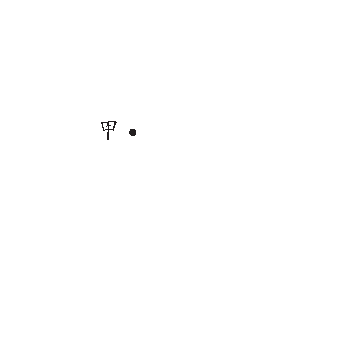
\includegraphics[angle=90]{eu1}
\end{center}

\cthm{第二界。線有長無廣。}\bcom{試如一平面,光照之,有光無光之間,不容一物,是線也。真平真圓相遇,其相遇處止有一點,行則止有一線。}
\bcom{線有直有曲。}
\begin{center}
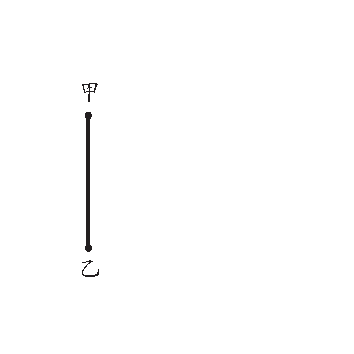
\includegraphics[angle=90]{eu2}
\end{center}

\cthm{第三界。線之界是點。}\ccom{凡線有界者,兩界必是點。}

\cthm{第四界。直線止有兩端,兩端之間上下更無一點。}\bcom{兩點之間至徑者,直線也。稍曲則繞而長矣。}\bcom{直線之中點能遮兩界。}\bcom{凡量遠近,皆用直線。}
\begin{center}
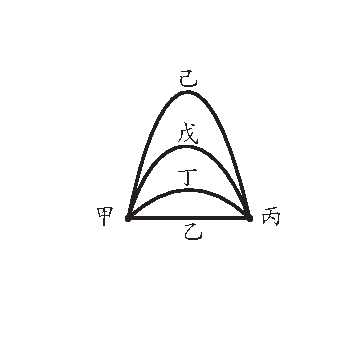
\includegraphics[angle=90]{eu3}
\end{center}
\bcom{甲乙丙是直線,甲丁丙、甲戊丙、甲己丙皆是曲線。}

\cthm{第五界。面者,止有長有廣。}\bcom{一體所見為面。}\bcom{凡體之影,極似於面。}\ccom{無厚之極。}\bcom{想一橫行,所留之迹,即成面也。}
\begin{center}
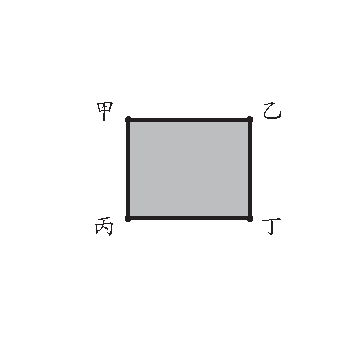
\includegraphics[angle=90]{eu4}
\end{center}

\cthm{第六界。面之界是線。}

\cthm{第七界。平面一面平,在界之內。}\bcom{平面中間線能遮兩界。}\bcom{平面者,諸方皆作直線。}
\begin{center}
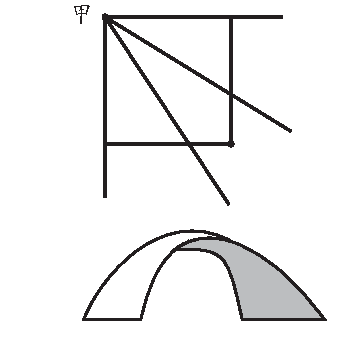
\includegraphics[angle=90]{eu5}
\end{center}
\bcom{試如一方面,用一直繩,施於一角,繞面運轉,不礙於空,是平面也。}\bcom{若曲面者,則中間線不能遮兩界。}

\cthm{第八界。平角者,兩直線於平面縱橫相遇交接處。}
\begin{center}
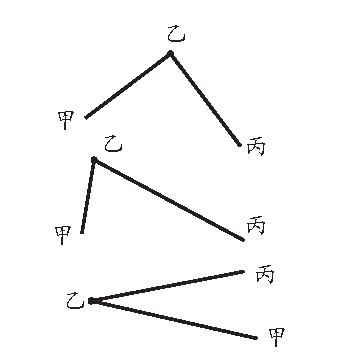
\includegraphics[angle=90]{eu6}
\end{center}
\bcom{凡言甲乙丙角,皆指平角。}
\begin{center}
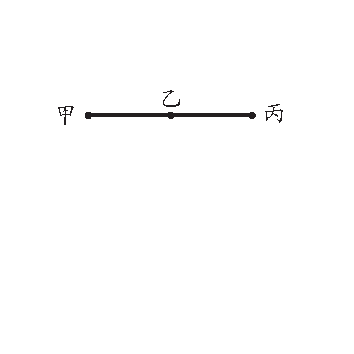
\includegraphics[angle=90]{eu7}
\end{center}
\bcom{如上,甲乙、乙丙二線平等,相遇不能作角。}
\begin{center}
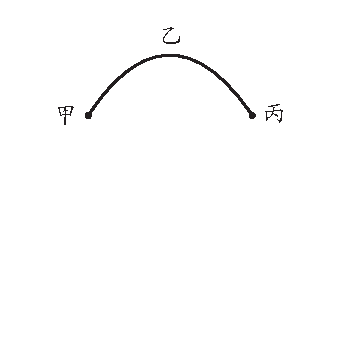
\includegraphics[angle=90]{eu8}
\end{center}
\bcom{如上,甲乙、乙丙二線雖相遇,不作平角,為是曲線。}\bcom{所謂角,止是兩線相映,不以線之大小較論。}

\cthm{第九界。直線相遇作角,為直線角。}\bcom{平地兩直線相遇為直線角。本書中所論,止是直線角。但作角有三等,今附著於此:一直線角,二曲線角,三雜線角。如下六圖。}
\begin{center}
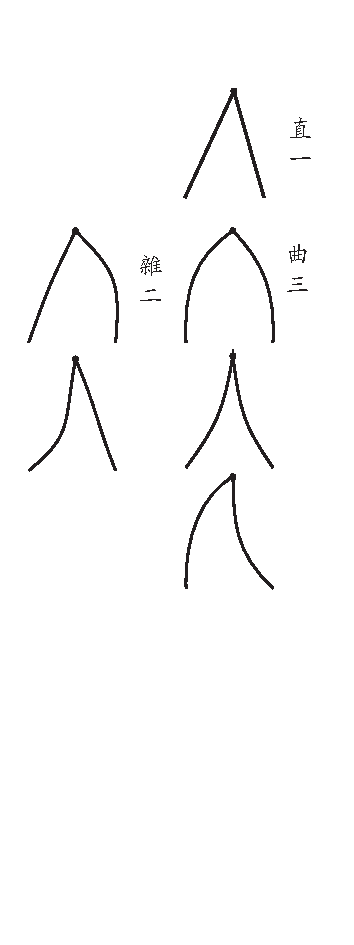
\includegraphics[angle=90]{eu9}
\end{center}

\cthm{第十界。直線垂於橫直線之上,若兩角等,必兩成直角,而直線下垂者,謂之橫線之垂線。}\bcom{量法常用直角及垂線。垂線加於橫線之上,必不作銳角及鈍角。}
\begin{center}
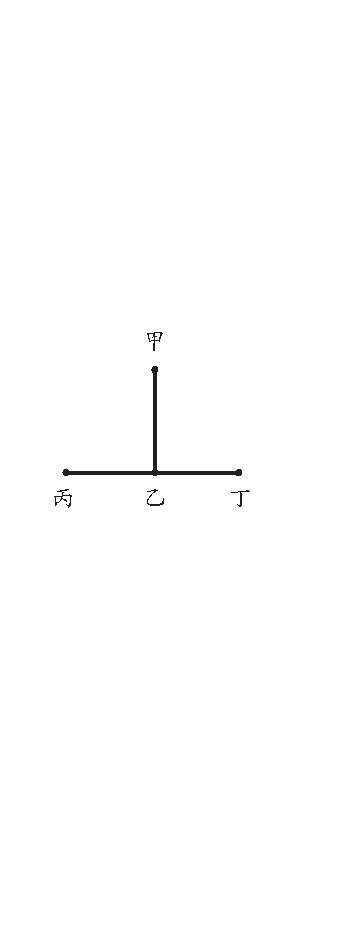
\includegraphics[angle=90]{eu10}
\end{center}
\bcom{若甲乙線至丙丁上,則乙之左右作兩角相等,為直角,而甲乙為垂線。}\bcom{若甲乙為橫線,則丙丁又為甲乙之垂線。何者?丙乙與甲乙相映雖止一直角,然甲線若垂下過乙,則丙線上下定成兩直角,所以丙乙亦為甲乙之垂線。}\ccom{如今用短尺,一縱一橫互相為直線,互相為垂線。}\bcom{凡直線上有兩角相連,是相等者,定俱直角,中間線為垂線。}\bcom{反用之,若是直角,則兩線定俱是垂線。}

\cthm{第十一界。凡角大于直角為鈍角。}
\begin{center}
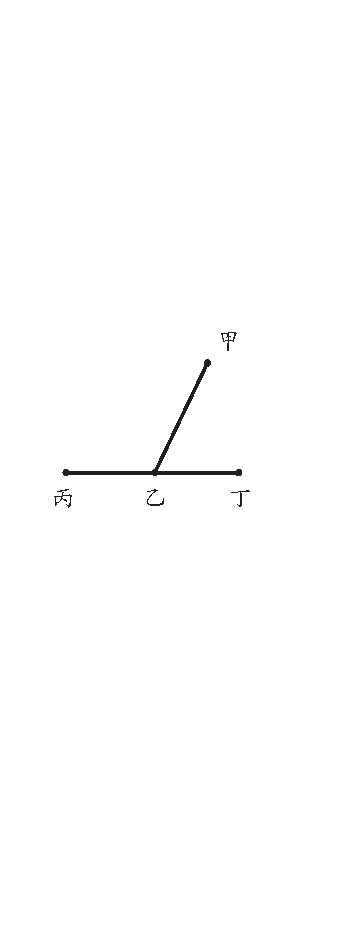
\includegraphics[angle=90]{eu11}
\end{center}
\bcom{如甲乙丙角與甲乙丁角不等,而甲乙丙大於甲乙丁,則甲乙丙為鈍角。}

\cthm{第十二界。凡角小於直角為銳角。}\bcom{如前圖甲乙丁是。}\bcom{通上三界,論之直角,一而已。鈍角、銳角,其大小不等,乃至無數。}\bcom{是後凡指言角者,俱用三字為識,其第二字即所指角也。 如前圖甲乙丙三字,第二乙字即所指鈍角。若言甲乙丁,即第二乙字是所指銳角。}

\cthm{第十三界。界者,一物之終始。}\bcom{今所論有三界:點為線之界,線為面之界,面為體之界,體不可為界。}

\cthm{第十四界。或在一界,或在多界之間為形。}\bcom{一界之形,如平圓、立圓等物。多界之形,如平方、立方及平立三角、六、八角等物。 圖見後卷。}

\cthm{第十五界。圜者,一形於平地,居一界之間,自界至中心作直線俱等。}
\begin{center}
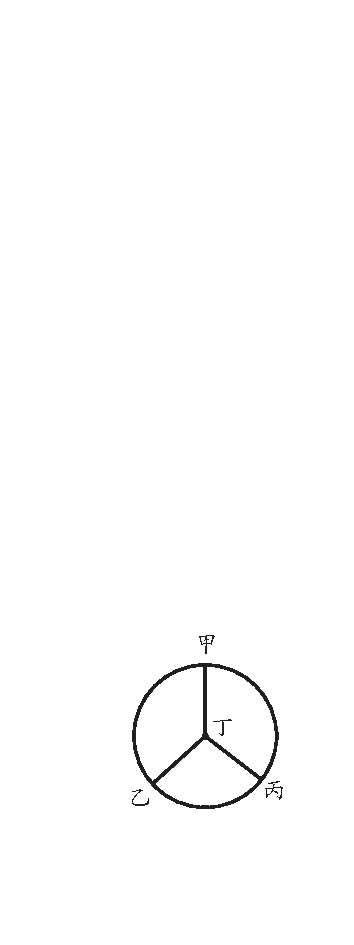
\includegraphics[angle=90]{eu12}
\end{center}
\bcom{若甲乙丙為圜,丁為中心,則自甲至丁與乙至丁、丙至丁,其線俱等。}\bcom{外圓線為圜之界,內形為圜。}\bcom{一說圜是一形,乃一線屈轉一周,復於元處所作,如上圖:甲丁線轉至乙丁,乙丁轉至丙丁,又至甲丁,復元處,其中形即成圜。}

\cthm{第十六界。圜之中處為圜心。}

\cthm{第十七界。自圜之一界作一直線過中心至他界為圜徑。徑分圜兩平分。}
\begin{center}
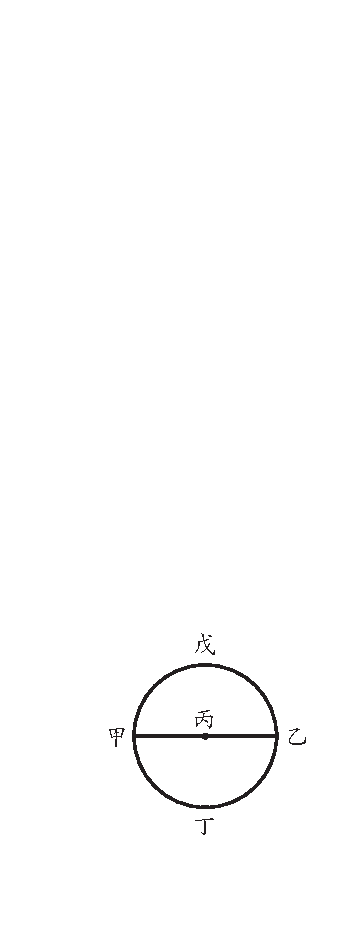
\includegraphics[angle=90]{eu13}
\end{center}
\bcom{甲丁乙戊圜。自甲至乙過丙作一直線,為圜徑。}

\cthm{第十八界。徑線與半圜之界所作形為半圜。}

\cthm{第十九界。在直線界中之形為直線形。}

\cthm{第二十界。在三直線界中之形為三邊形。}

\cthm{第二十一界。在四直線界中之形為四邊形。}

\cthm{第二十二界。在多直線界中之形為多邊形。}\ccom{五邊以上俱是。}

\cthm{第二十三界。三邊形三邊線等為平邊三角形。}
\begin{center}
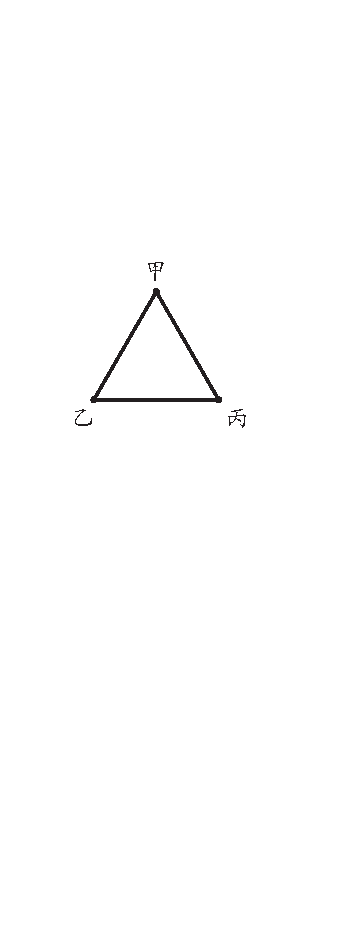
\includegraphics[angle=90]{eu14}
\end{center}

\cthm{第二十四界。三邊形有兩邊線等為兩邊等三角形。}\ccom{或銳或鈍。}
\begin{center}
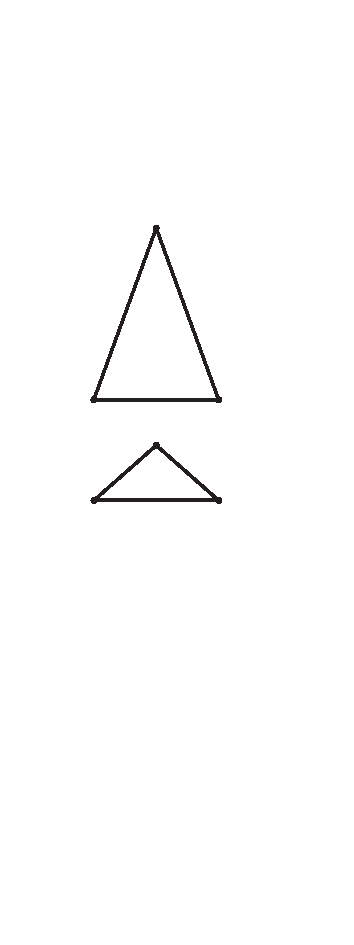
\includegraphics[angle=90]{eu15}
\end{center}

\cthm{第二十五界。三邊形三邊線俱不等為三不等三角形。}
\begin{center}
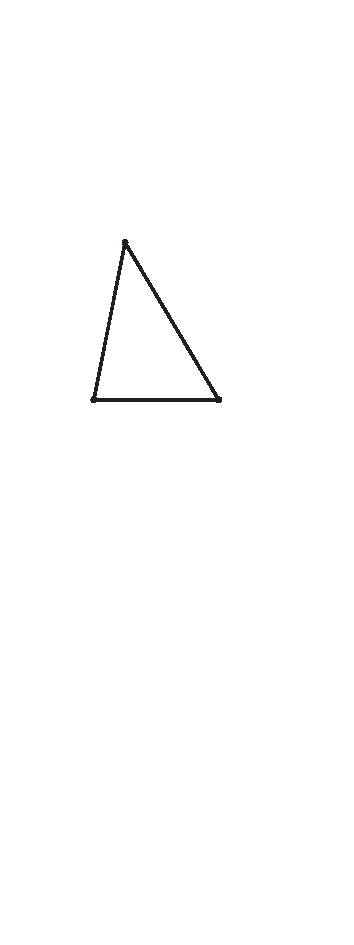
\includegraphics[angle=90]{eu16}
\end{center}

\cthm{第二十六界。三邊形在一直角為三邊直角形。}
\begin{center}
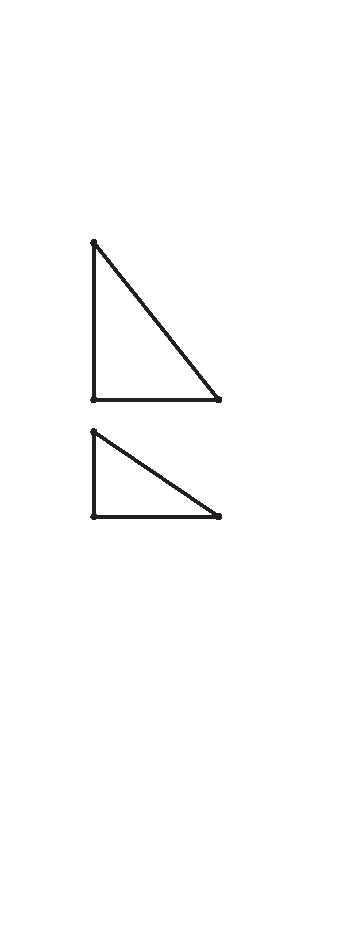
\includegraphics[angle=90]{eu17}
\end{center}

\cthm{第二十七界。三邊形有一鈍角為三邊鈍角形。}
\begin{center}
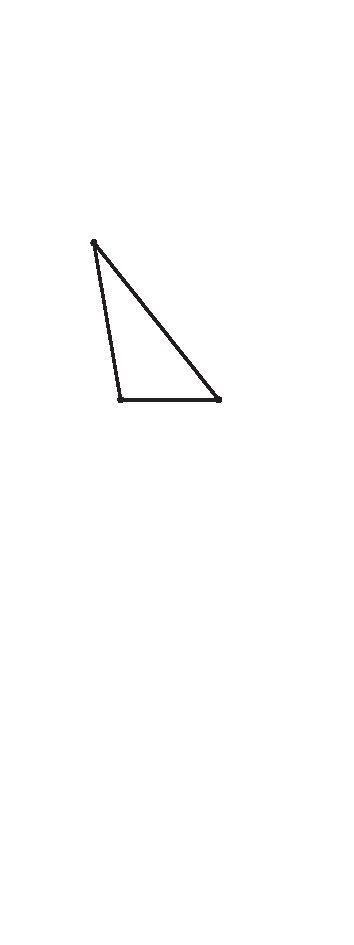
\includegraphics[angle=90]{eu18}
\end{center}

\cthm{第二十八界。三邊形有三銳角為三邊各銳角形。}\bcom{凡三邊形,恒以在下者為底,在上二邊為腰。}

\cthm{第二十九界。四邊形四邊線等而角直為直角方形。}
\begin{center}
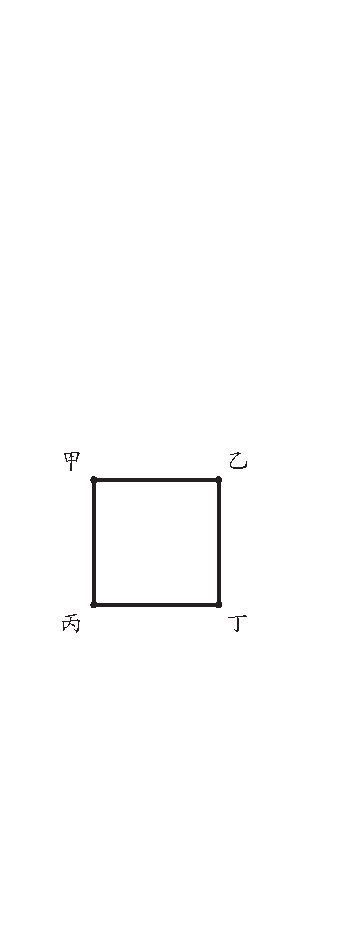
\includegraphics[angle=90]{eu19}
\end{center}

\cthm{第三十界。直角形其角俱是直角,其邊兩兩相等。}
\begin{center}
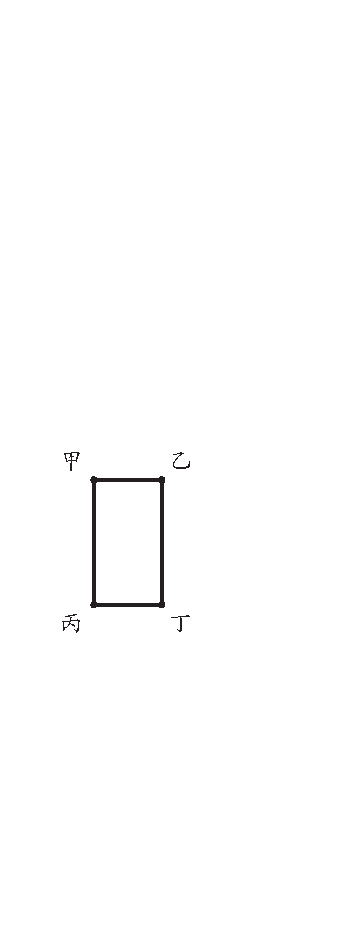
\includegraphics[angle=90]{eu20}
\end{center}
\bcom{如上甲乙丙丁形。甲乙邊與丙丁邊自相等,甲丙與乙丁自相等。}

\cthm{第三十一界。斜方形四邊等,俱非直角。}
\begin{center}
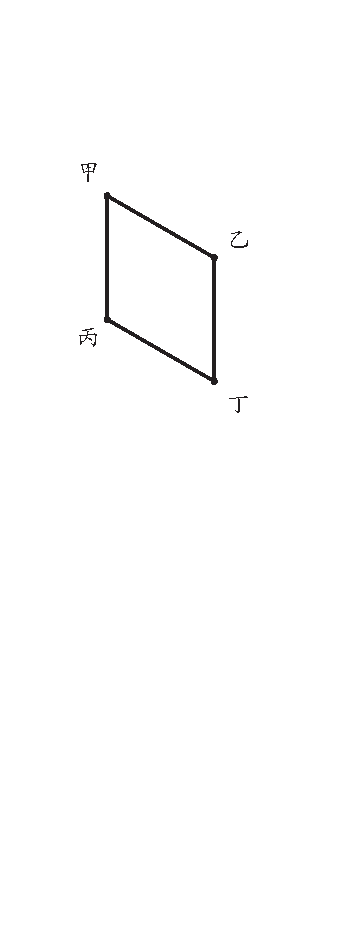
\includegraphics[angle=90]{eu21}
\end{center}

\cthm{第三十二界。長斜方形其邊兩兩相等,俱非直角。}
\begin{center}
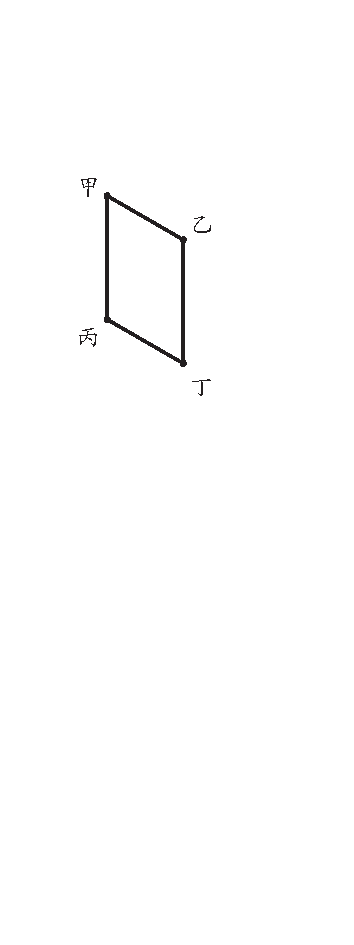
\includegraphics[angle=90]{eu22}
\end{center}

\cthm{第三十三界。以上方形四種謂之有法四邊形。四種之外他方形皆謂之無法四邊形。}
\begin{center}
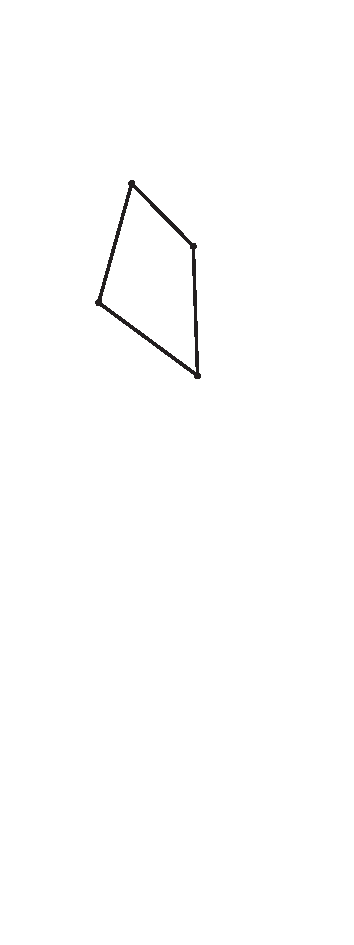
\includegraphics[angle=90]{eu23}
\end{center}

\cthm{第三十四界。兩直線於同面行,至無窮不相離亦不遇為平行線。}
\begin{center}
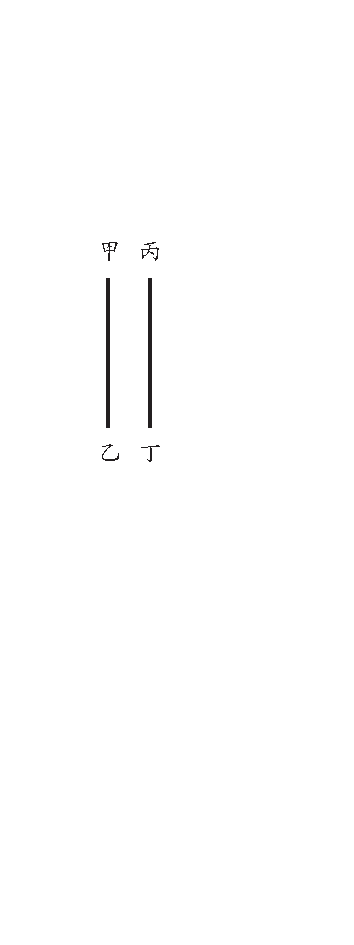
\includegraphics[angle=90]{eu24}
\end{center}

\cthm{第三十五界。一形每兩邊有平行線為平行線方形。}
\begin{center}
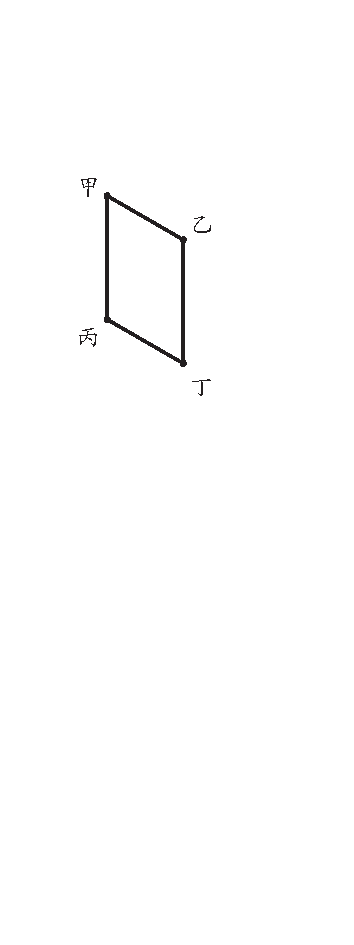
\includegraphics[angle=90]{eu22}
\end{center}

\cthm{第三十六界。凡平等線方形,若於兩對角作一直線,其直線為對角線。又於兩邊縱橫各作一平等線,其兩平等線與對角線交羅相遇,即此形分為四平行線方形,其兩形有對角線者為角線方形,其兩形無對角線者為餘方形。}
\begin{center}
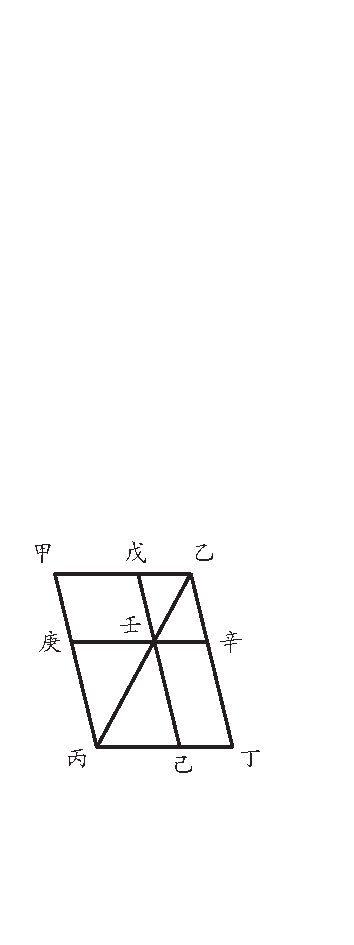
\includegraphics[angle=90]{eu25}
\end{center}
\bcom{甲乙丁丙方形於丙乙兩角作一線,為對角線,又依乙丁平行作戊己線,依甲乙平行作庚辛線,其對角線與戊己、庚辛兩線交羅相遇於壬,即作大小四平行線方形矣,則庚壬己丙及戊城辛乙兩方謂之角線方形,而甲庚壬戊及壬己丁辛謂之餘方形。}

\subsection*{\mincho 求作四則}
\addcontentsline{toc}{subsection}{求作四則}

求作者,不得言不可作。

\cthm{第一求。自此點至彼點求作一直線。}\bcom{此求亦出上篇。葢自此點直行至彼點,即是直線。自甲至乙或至丙、至丁,俱可作直線。}
\begin{center}
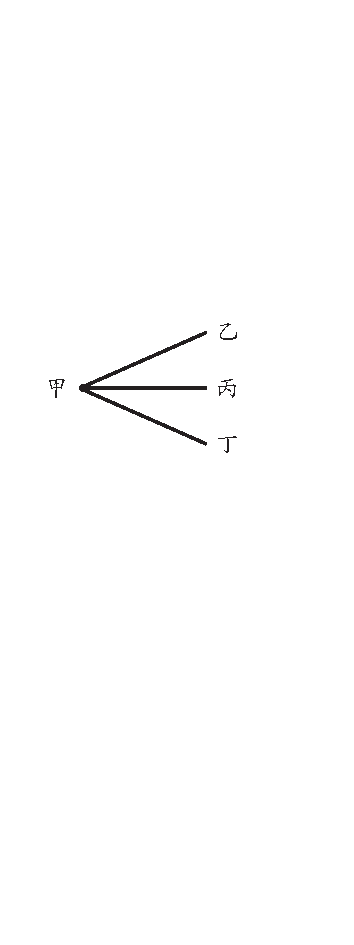
\includegraphics[angle=90]{eu26}
\end{center}

\cthm{第二求。一有界直線,求從彼界直行引長之。}
\begin{center}
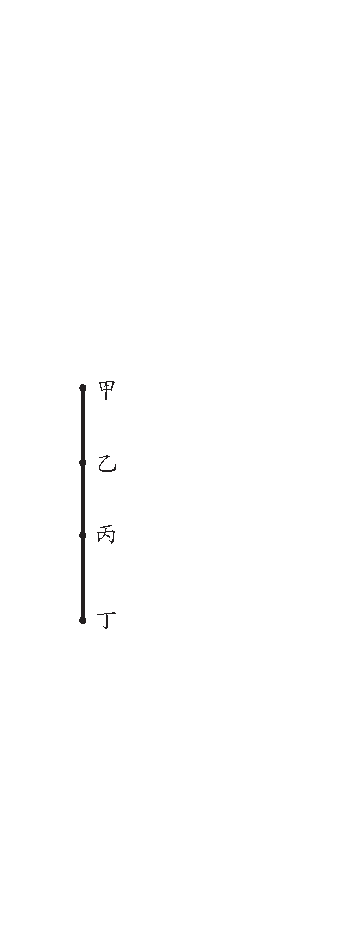
\includegraphics[angle=90]{eu27}
\end{center}
\bcom{如甲乙線。從乙引至丙,或引至丁,俱一直行。}

\cthm{第三求。不論大小,以點為心,求作一圜。}
\begin{center}
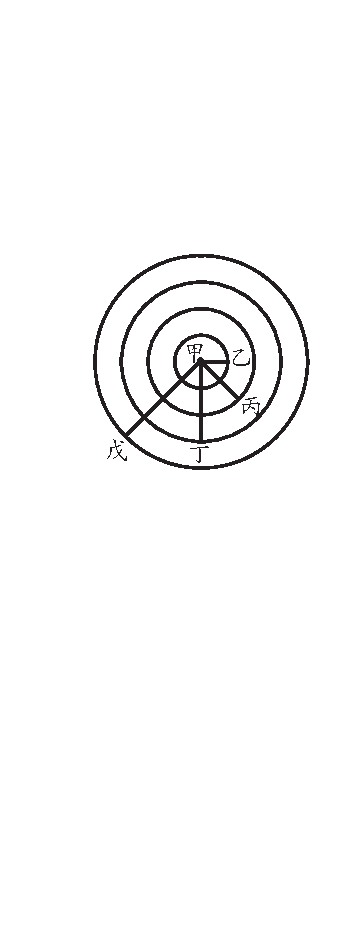
\includegraphics[angle=90]{eu28}
\end{center}

\cthm{第四求。設一度於此,求作彼度,較此度或大或小。}\ccom{凡言度者,或線、或面、或體皆是。}\bcom{或言:較小作大可作,較大作小不可作。何者?小之至極,數窮盡故也。此說非是。凡度與數不同。數者,可以長不可以短。長數無窮,短數有限,如百數減半成五十,減之又減至一而止,一以下不可損矣。自百以上,增之可至無窮,故曰:可長不可短也。度者可以長亦可以短。長者,增之可至無窮;短者,減之亦復無盡。嘗見莊子稱一尺之棰,日取其半,萬世不竭,亦此理也。何者?自有而分,不免為有。若減之可盡,是有化為無也。有化為無,猶可言也。令已分者更復合之,合之又合,仍為尺棰,是始合之初,兩無能並為一有也。兩無能並為一有不可言也。}

\subsection*{\mincho 公論十九則}
\addcontentsline{toc}{subsection}{公論十九則}

公論者,不可疑。

\cthm{第一論。設有多度,彼此俱與他等,則彼與此自相等。}

\cthm{第二論。有多度等。若所加之度等,則合并之度亦等。}

\cthm{第三論。有多度等。若所減之度等,則所存之度亦等。}

\cthm{第四論。有多度不等。若所加之度等,則合并之度不等。}

\cthm{第五論。有多度不等。若所減之度等,則所存之度不等。}

\cthm{第六論。有多度,俱倍於此度,則彼多度俱等。}

\cthm{第七論。有多度,俱半於此度,則彼多度亦等。}

\cthm{第八論。有二度,自相合,則二度必等。}\ccom{以一度加一度之上。}

\cthm{第九論。全大於其分。}\ccom{如一尺大於一寸。寸者,全尺中十分中之一分也。}

\cthm{第十論。直角俱相等。}\ccom{見界說十。}

\cthm{第十一論。有二橫直线,或正或偏,任加一縱線,若三線之間同方兩角小於兩直角,則此二橫直線愈長愈相近,必至相遇。甲乙、丙丁二橫直線,任意作一戊己縱線,或正或偏,若戊己線同方兩角俱小於直角,或并之小於兩直角,則甲乙丁線愈長愈相近,必有相遇之處。}
\begin{center}
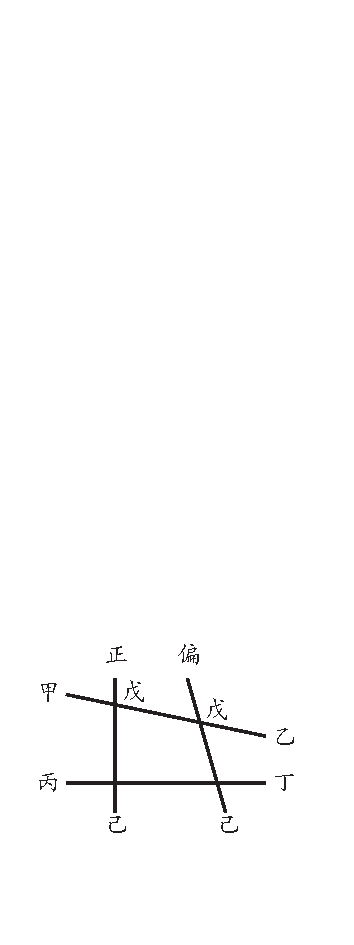
\includegraphics[angle=90]{eu29}
\end{center}
\bcom{欲明此理,宜察平行線不得相遇者。\ccom{界說卅四。}加一垂線,即三線之間定為直角,便知此論。兩角小於直角者,其行不得不相遇矣。}

\cthm{第十二論。兩直線不能為有界之形。}
\begin{center}
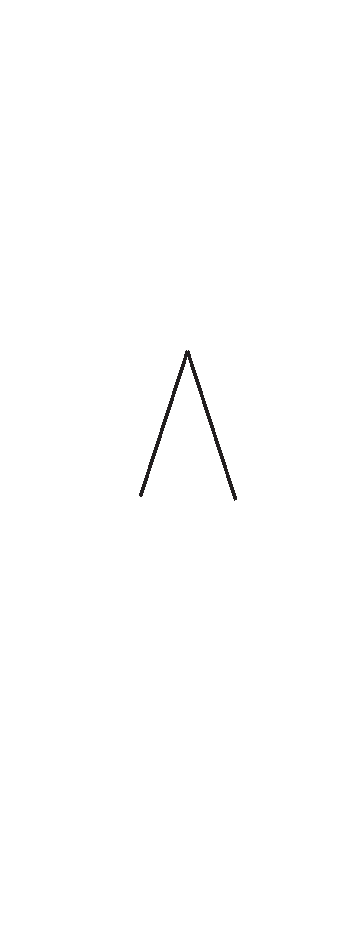
\includegraphics[angle=90]{eu30}
\end{center}

\cthm{第十三論。兩直線止能於一點相遇。}
\begin{center}
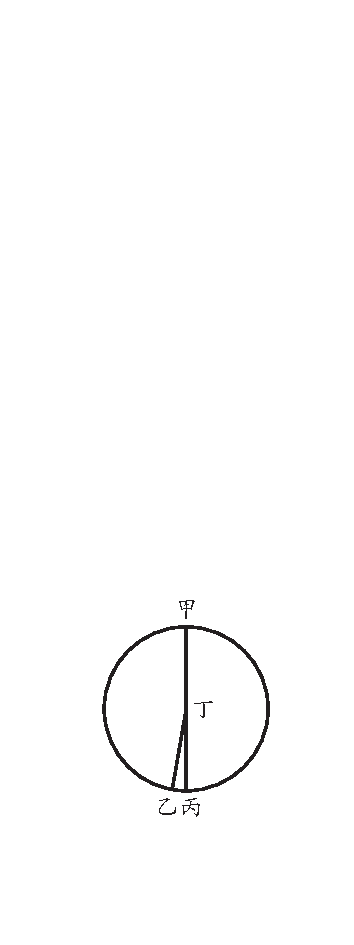
\includegraphics[angle=90]{eu31}
\end{center}
\bcom{如云線長界近,相交不止一點,試於丙乙二界各出直線,交於丁。假令其交不止一點,當引至甲,則甲丁乙宜為甲丙乙圜之徑,而甲丁丙亦如之。\ccom{界說十七。}夫甲丁乙,圜之右半也,而甲丁丙亦右半也。\ccom{界說十七。}甲丁乙為全,甲丁丙為其分,而俱稱右半,是全與其分等也。\ccom{本篇九。}}

\cthm{第十四論。有幾何度等。若所加之度各不等,則合并之差與所加之差等。}
\begin{center}
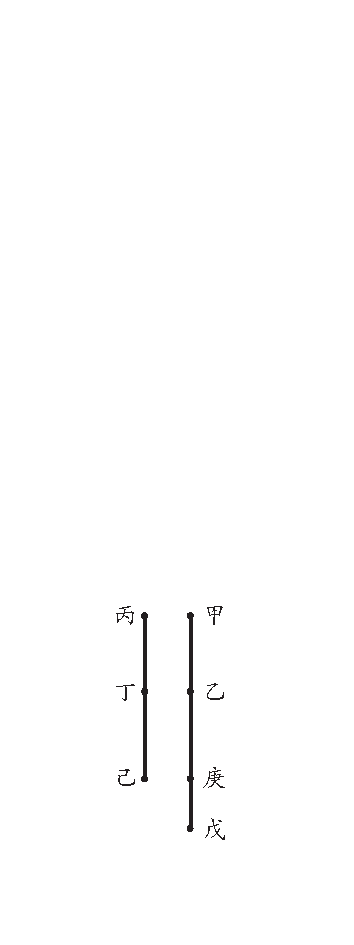
\includegraphics[angle=90]{eu32}
\end{center}
\bcom{甲乙丙丁線等于甲乙加乙戊於丙丁加丁己,則甲戊大於丙己者,庚戊線也,而乙戊大於丁己亦如之。}

\cthm{第十五論。有幾何度不等。若所加之度等,則合并所贏之度與元所贏之度等。}
\begin{center}
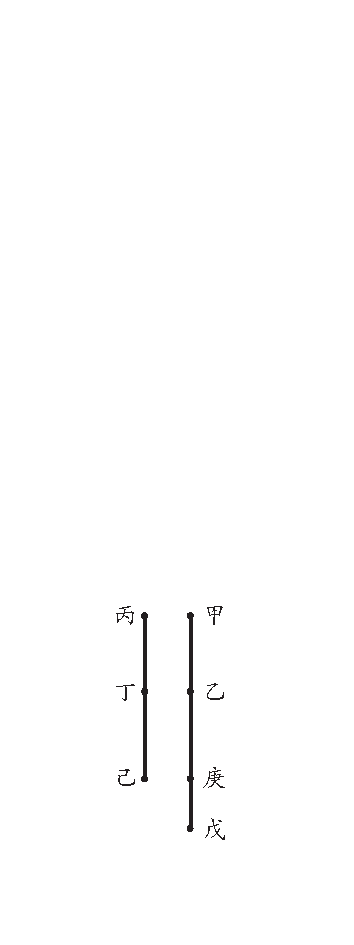
\includegraphics[angle=90]{eu32}
\end{center}
\bcom{如上圖。反說之,戊乙、己丁線不等於戊乙加乙甲於己丁加丁丙,則戊甲大於己丙者,戊庚線也,而戊乙大於己丁亦如之。}

\cthm{第十六論。有幾何度等。若所減之度不等,則餘度所贏之度與減去所贏之度等。}
\begin{center}
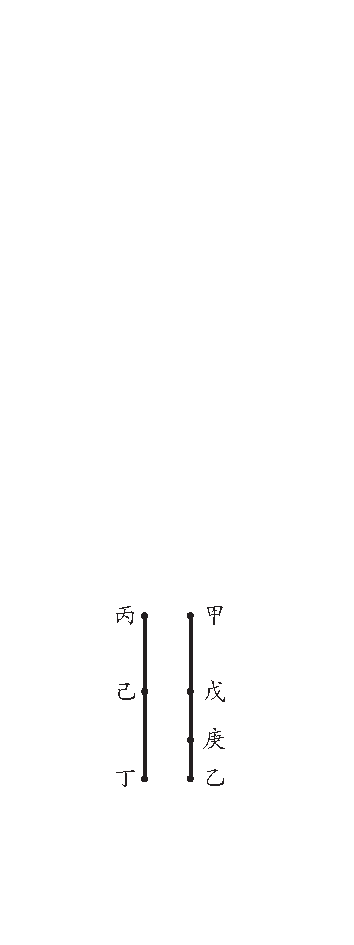
\includegraphics[angle=90]{eu33}
\end{center}
\bcom{甲乙丙丁線等於甲乙減戊乙於丙丁減己丁,則乙戊大於丁己者,庚戊也,而丙己大於甲戊亦如之。}

\cthm{第十七論。有幾何度不等。若所減之度等,則餘度所贏之度與元所贏之度等。}
\begin{center}
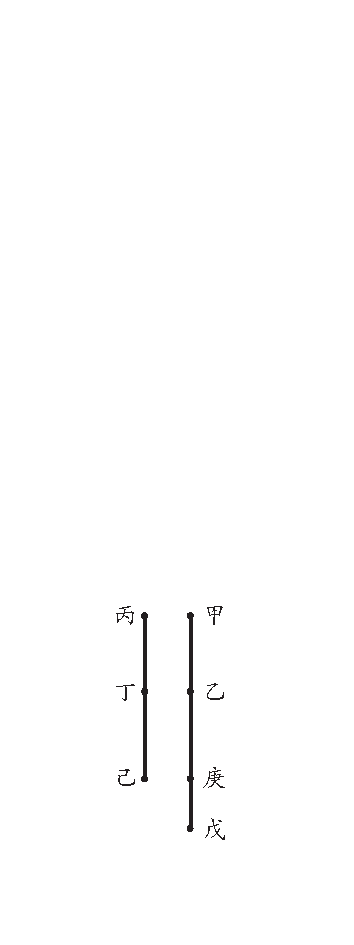
\includegraphics[angle=90]{eu32}
\end{center}
\bcom{如十四論,反說之。甲戊丙己線不等於甲戊減甲乙於丙己減丙丁,則乙戊長於丁己者,亦庚戊也,與甲戊長於丙己者等矣。}

\cthm{第十八論。全與諸分之并等。}

\cthm{第十九論。有二全度,此全倍於彼全。若此全所減之度倍於彼全所減之度,則此較亦倍於彼較。}\ccom{相減之餘曰較。}\bcom{如此度二十,彼度十,於二十減六,於十減三,則此較十四,彼較七。}

\section*{\mincho 幾何原本卷一}
\addcontentsline{toc}{section}{卷一}

\cthm{第一題。于有界直線上,求立平邊三角形。}
\begin{center}
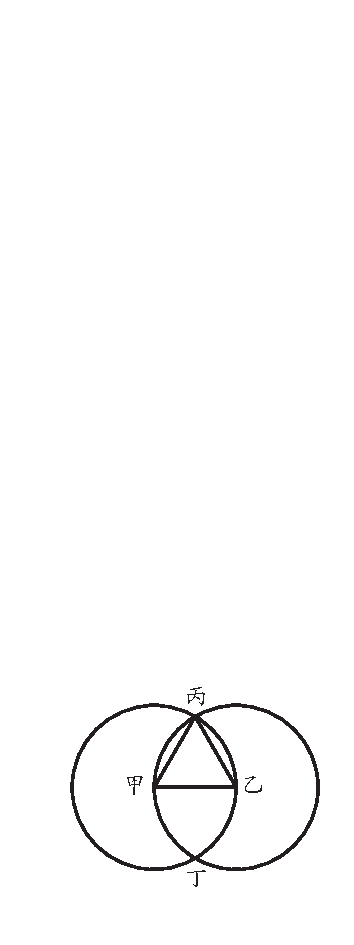
\includegraphics[angle=90]{eu34}
\end{center}
\bcom{法曰:甲乙直線上求立平邊三角形。先以甲為心,乙為界,作丙乙丁圜,次以乙為心,甲為界,作丙甲丁圜。兩圜相交于丁末。自甲至丙,丙至乙,各作直線,即甲乙丙為平邊三角形。}\bcom{論曰:以甲為心,至圜之界,其甲乙線與甲丙、甲丁線等。以乙為心,則乙甲線與乙丙、乙丁線亦等。何者?凡為圜,自心至界,各線俱等故。\ccom{界說十五。}既乙丙等于乙甲,而甲丙亦等于甲乙,即甲丙亦等于乙丙。\ccom{公論一。}三邊等,如所求。\ccom{凡論有二種,此以是為論者正論也。下倣此。}}
\begin{center}
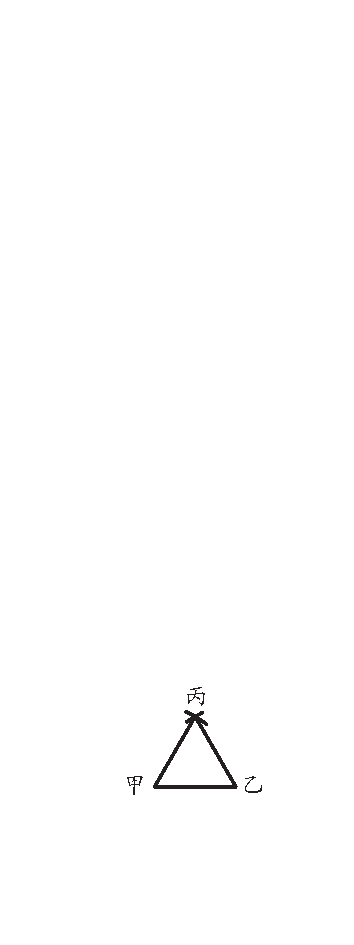
\includegraphics[angle=90]{eu35}
\end{center}
\bcom{其用法不心作兩圜。但以甲為心,乙為界,作近丙一短界線;乙為心,甲為界,亦如之。兩短界線交處即得丙。}\bcom{諸三角形,俱推前用法作之。\ccom{詳本篇廿二。}}

\cthm{第二題。一直線,線或內或外有一點。求以點為界作直線,與元線等。}
\begin{center}
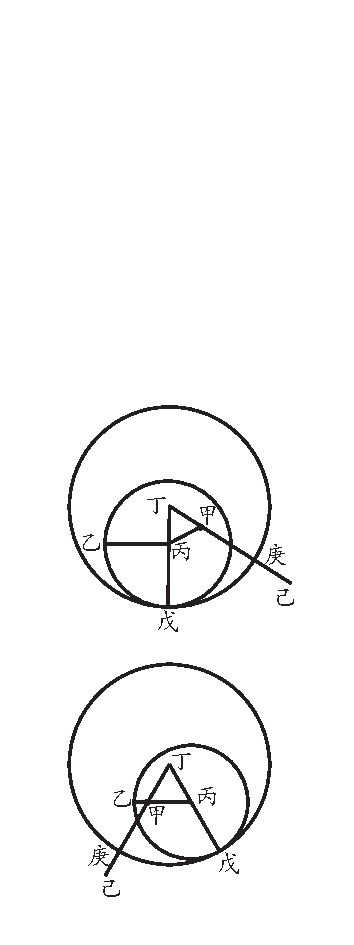
\includegraphics[angle=90]{eu36}
\end{center}
\bcom{法曰:有甲點及乙丙線,求以甲為界,作一線,與乙丙等。先以丙為心,乙為界,\ccom{乙為心,丙為界亦可作。}作丙乙圜。\ccom{第三求。}次觀甲點。若在丙乙之外,則自甲至丙作甲丙線。\ccom{第一求。}如上前圖。或甲在丙乙之內,則截取甲至丙一分線,如上圖。兩法俱以甲丙線為底,任于上下作甲丁丙平邊三角形。\ccom{本篇一。}次自三角形兩腰線引長之。\ccom{第二求。}其丁丙引至丙乙圜界而止,為丙戊線;其丁甲引之出丙乙圜,外稍長,為甲己線。末以丁為心,戊為界,作丁戊圜,其甲己線與丁戊圜相交于庚,即甲庚線,與乙丙線等。}\bcom{論曰:丁戊、丁庚線同以丁為心,戊庚為界,故等。\ccom{界說十五。}于丁戊線減丁丙,丁庚線減丁甲,其所減兩腰線等,則所存亦等。\ccom{公論三。}夫丙戊與丙乙同以丙為心,戊乙為界,亦等。\ccom{界說十五。}即甲庚與丙乙等。\ccom{公論一。}}\bcom{若所設。甲點即在丙乙線之一界,其法尤易。假如點在丙,即以丙為心,作乙戊圜,從丙至戊即所求。}

\cthm{第三題。兩直線,一長一短。求于長線減去短線之度。}
\begin{center}
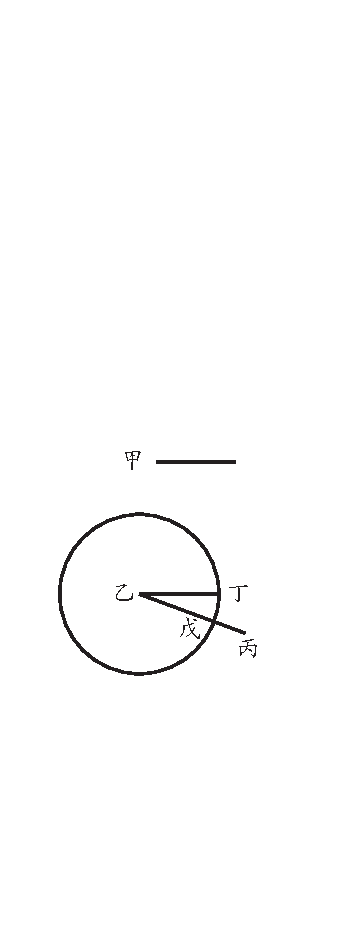
\includegraphics[angle=90]{eu37}
\end{center}
\bcom{法曰:甲短線,乙丙長線,求于乙丙減甲。先以甲為度,從乙引至別界,作乙丁線;\ccom{本篇二。}次以乙為心,丁為界,作圜。\ccom{第三求。}圜界與乙丙交于戊,即乙戊與等。甲之乙丁等,葢乙丁、乙戊同心同圜故。\ccom{界說十五。}}

\cthm{第四題。兩三角形,若相當之兩腰線各等,各兩腰線間之角等,則兩底線必等,而兩形亦等。其餘各兩角相當者俱等。}
\begin{center}
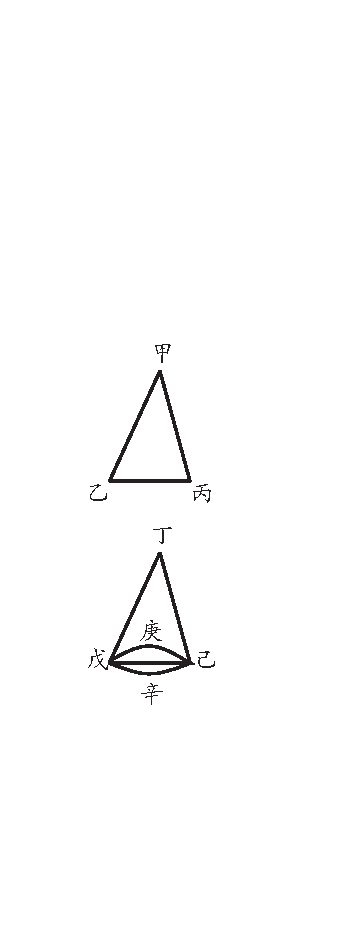
\includegraphics[angle=90]{eu38}
\end{center}
\bcom{解曰:甲乙丙、丁戊己兩三角形之甲與丁兩角等,甲丙與丁己兩線,甲乙與丁戊兩線各等。題言乙丙與戊己兩底線必等,而兩三角形亦等。甲乙丙與丁戊己兩角,甲丙乙與丁己戊兩角俱等。}\bcom{論曰:如云乙丙與戊己不等,即令將甲角置丁角之上,兩角必相合,無大小。甲丙與丁己、甲乙與丁戊亦必相合,無大小。\ccom{公論八。}此二俱等,而云乙丙與戊己不等,必乙丙底或在戊己之上,為庚,或在其下,為辛矣。戊己既為直線,而戊庚己又為直線,則兩線當別作一形,是兩線能相合為形也。辛倣此。\ccom{公論十二。此以非為論者,駁論也。下倣此。}}

\cthm{第五題。三角形若兩腰等,則底線兩端之兩角等,而兩腰引出之其底之外兩角亦等。}
\begin{center}
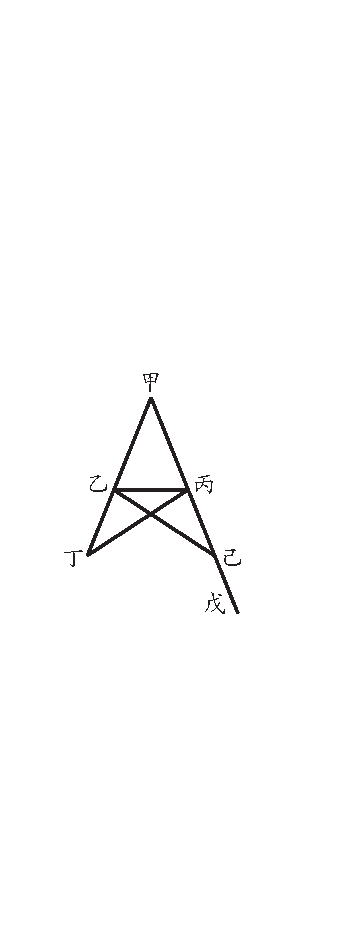
\includegraphics[angle=90]{eu39}
\end{center}
\bcom{解曰:甲乙丙三角形,其甲丙與甲乙兩腰等。題言甲丙乙與甲乙丙兩角等,又自甲丙線任引至戊,甲乙線任引至丁,其乙丙戊與丙乙丁兩外角亦等。}\bcom{論曰:試如甲戊線稍長,即從甲戊截取一分,與甲丁等,為甲己。\ccom{本篇三。}次自丙至丁,乙至己,各作直線。\ccom{第一求。}即甲己乙、甲丁丙兩三角形必等。何者?此兩形之甲角同,己與甲丁兩腰又等,甲乙與甲丙兩腰又等,則其底丙丁與乙己必等,而底線兩端相當之各兩角亦等矣。\ccom{本篇四。}又乙丙己與丙乙丁兩三角形亦等。何者?此兩形之丙丁乙與乙己丙兩角既等,\ccom{本論。}而甲己、甲丁兩腰各減相等之甲丙、甲乙線,即所存丙己、乙丁兩腰又等。\ccom{公論三。}丙丁與乙己兩底又等,\ccom{本論。}又乙丙同腰,即乙丙丁與丙乙己兩角亦等也。則丙之外乙丙己角與乙之外丙乙丁角必等矣。\ccom{本篇四。}次觀甲乙己與甲丙丁兩角既等于甲乙己減丙乙己角,甲丙丁減乙丙丁角,則所存甲丙乙與甲乙丙兩角必等。\ccom{公論三。}}
\begin{center}
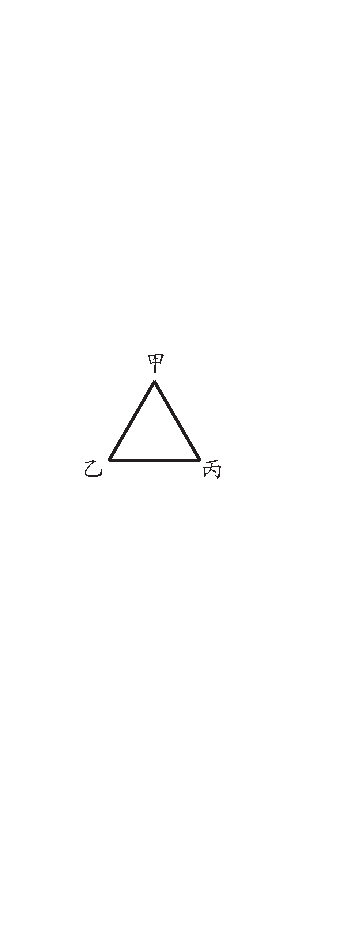
\includegraphics[angle=90]{eu40}
\end{center}
\bcom{增:從前形知,三邊等形,其三角俱等。}

\cthm{第六題。三角形若底線兩端之角等,則兩腰亦等。}
\begin{center}
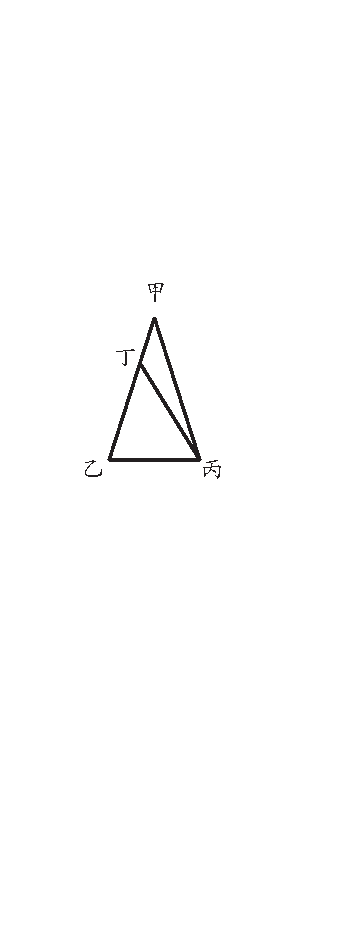
\includegraphics[angle=90]{eu41}
\end{center}
\bcom{解曰:甲乙丙三角形,其甲乙丙與甲丙乙兩角等。題言甲乙與甲丙兩腰亦等。}\bcom{論曰:如云兩腰線不等,而一長一短,試辯之。若甲乙為長線,即令比甲丙線截去所長之度,為乙丁線,而乙丁與甲丙等。\ccom{本篇三。}次自丁至丙作直線,則本形成兩三角形,其一為甲乙丙,其一為丁乙丙。而甲乙丙全形與丁乙丙分形同也。是全與其分等也。\ccom{公論九。}何者?彼言丁乙丙分形之乙丁與甲乙丙全形之甲丙兩線既等,丁乙丙分形之乙丙與甲乙丙全形之乙丙又同線,而元設丁乙丙與甲丙乙兩角等,則丁乙丙與甲乙丙兩形亦等也。\ccom{本篇四。}是全與其分等也。故底線兩端之兩角等者,兩腰必等也。}

\cthm{第七題。一線為底,出兩腰線,其相遇止有一點,不得別有腰線與元腰線等而于此點外相遇。}
\begin{center}
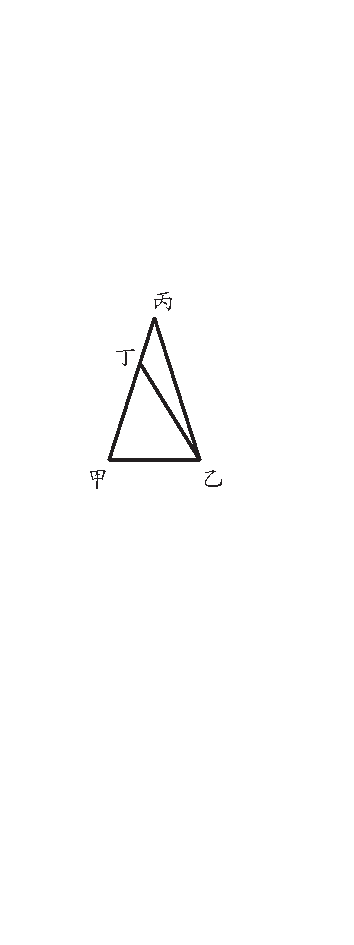
\includegraphics[angle=90]{eu42}
\end{center}
\bcom{解曰:甲乙線為底,于甲于乙各出一線,至丙點相遇。題言此為一定之處,不得于甲上更出一線,與甲丙等,乙上更出一線,與乙丙等,而不于丙相遇。}
\begin{center}
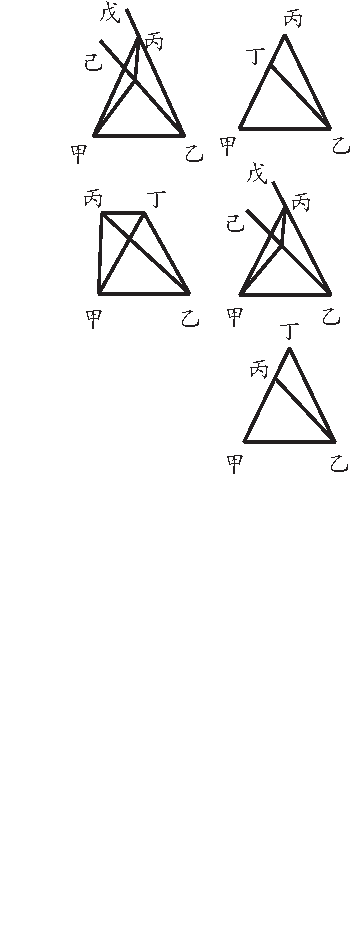
\includegraphics[angle=90]{eu43}
\end{center}
\bcom{論曰:若言有別相遇于丁者,即問丁當在丙內邪?丙外邪?若言丁在丙內,則有二說,俱不可通。何者?若言丁在丙元線之內,則如第一圖,丁在丙兩界之間矣。如此,即甲丁是甲丙之分,而云甲丙與甲丁等也,是全與其分等也。\ccom{公論九。}若言丁在甲丙乙三角頂間,則如第二圖,丁在甲丙乙之間矣。即令自丙至丁,作丙丁線,而乙丁丙、甲丁丙又成兩三角形。次從乙丁引出至己,從乙丙引出至戊,則乙丁丙形之乙丁、乙丙兩腰等者,其底線兩端之兩角乙丁丙、乙丙丁宜亦等也。其底之外兩角己丁丙、戊丙丁宜亦等也。\ccom{本篇五。}而甲丁丙形之甲丁、甲丙兩腰等者,其底線兩端之兩角甲丙丁、甲丁丙宜亦等也。\ccom{本篇五。}夫甲丙丁角本小于戊丙丁角,而為其分,今言甲丁丙與甲丙丁兩角等,則甲丁丙亦小于戊丙丁矣。何況己丁丙又甲丁丙之分,更小于戊丙丁,可知。何言底外兩角等乎?若言丁在丙外,又有三說,俱不可通。何者?若言丁在甲丙元線外,是丁甲即在丙甲元線之上,則甲丙與甲丁等矣。即如上第一說駁之。若言丁在甲丙乙三角頂外,即如上第二說駁之。若言丁在丙外,而後出二線,一在三角形內,一在其外。甲丁線與乙丙線相交,如第五圖。即令將丙丁相聯,作直線,是甲丁丙又成一三角形,而甲丙丁宜與甲丁丙兩角等也。\ccom{本篇五。}夫甲丁丙角本小于丙丁乙角,而為其分據,如彼論則甲丙丁角亦小于丙丁乙角矣。又丙丁乙亦成一三角形,而丙丁乙宜與丁丙乙兩角等也。\ccom{本篇五。}夫丁丙乙角本小于甲丙丁角,而為其分,據如彼論,則丙丁乙角亦小于甲丙丁角矣。此二說者,豈不自相戾乎?}

\cthm{第八題。兩三角形,若相當之兩腰各等,兩底亦等,則兩腰間角必等。}
\begin{center}
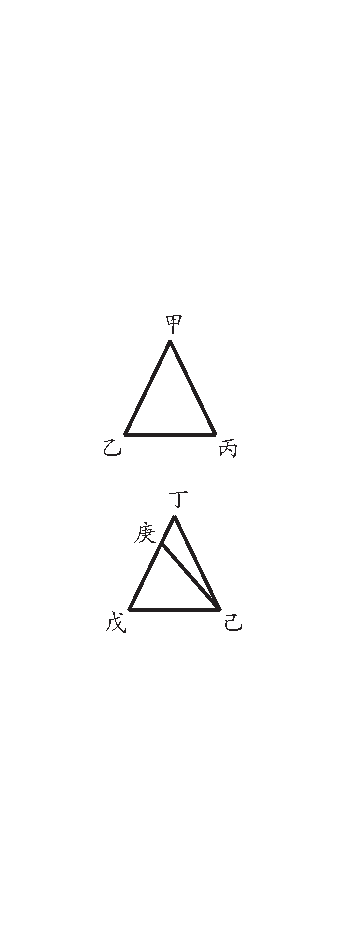
\includegraphics[angle=90]{eu44}
\end{center}
\bcom{解曰甲乙丙、丁戊己兩三角形,其甲乙與丁戊兩腰,甲丙與丁己兩腰各等,乙丙與戊己兩底亦等。題言甲與丁兩角必等。}
\begin{center}
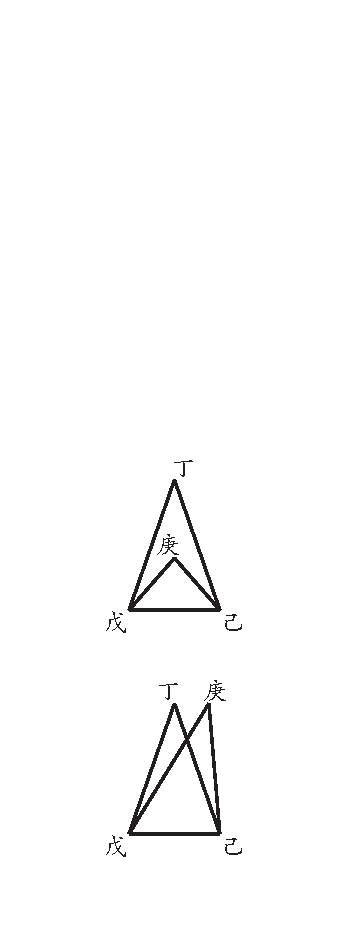
\includegraphics[angle=90]{eu45}
\end{center}
\bcom{論曰:試以丁戊己形加于甲乙丙形之上,問丁角在甲角上邪?否邪?若在上,即兩角等矣。\ccom{公論八。}或謂不然,乃在于庚,即問庚當在丁戊線之內邪?或在三角頂之內邪?或在三角頂之外邪?皆依前論駁之。\ccom{本篇七。}}\bcom{系:本題止論甲丁角。若旋轉,依法論之,即三角皆同。可見凡線等,則角必等,不可疑也。}

\cthm{第九題。有直線角。求兩平分之。}
\begin{center}
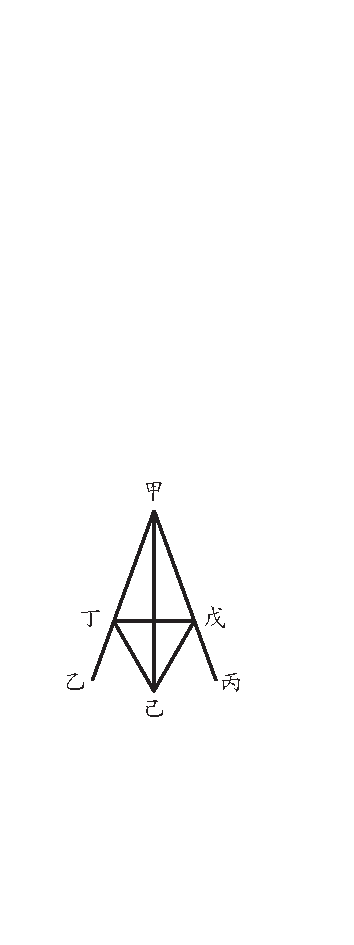
\includegraphics[angle=90]{eu46}
\end{center}
\bcom{法曰:乙甲丙角。求兩平分之。先于甲乙線任截一分,為甲丁。\ccom{本篇三。}次于甲丙亦截甲戊,與甲丁等次。自丁至戊作直線。次以丁戊為底,立平邊三角形,\ccom{本篇一。}為丁戊己形。末自己至申,作直線,即乙甲丙角為兩平分。}\bcom{論曰:丁甲己與戊甲己兩三角形之甲丁與甲戊兩線等,甲己同是一線,戊己與丁己兩底又等。\ccom{何言兩底等?初從戊丁底作此三角平形,此二線為腰,各等戊丁故。}則丁甲己與戊甲己兩角必等。\ccom{本篇八。}}
\begin{center}
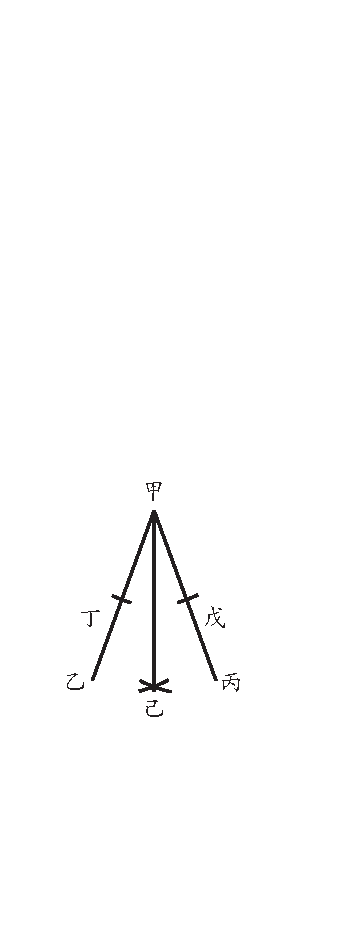
\includegraphics[angle=90]{eu47}
\end{center}
\bcom{用法:如上。截取甲丁、甲戊,即以丁為心,向乙丙間任作一短界線。次用元度,以戊為心,亦如之。兩界線交處得己。\ccom{本篇一。}}

\cthm{第十題。一有界線,求兩平分之。}
\begin{center}
\includegraphics[angle=90]{eu48}
\end{center}
\bcom{法曰:甲乙線求兩平分。先以甲乙為底,作甲乙丙兩邊等三角形。\ccom{本篇一。}次以甲丙乙角兩平分之,\ccom{本篇九。}等丙丁直線,即分甲乙于丁。}\bcom{論曰:丙丁乙、丙丁甲兩三角形之丙乙、丙甲兩腰等,而丙丁同線,甲丙丁與乙丙丁兩角又等。\ccom{本篇九。}則甲丁與乙丁兩線必等。\ccom{本篇四。}}
\begin{center}
\includegraphics[angle=90]{eu49}
\end{center}
\bcom{用法。以甲為心,任用一度,但須長于甲乙線之半,向上下各作一短界線。次用元度以乙為心,亦如之。兩界線交處即丙丁。末作丙丁直線,即分甲乙于戊。}

\cthm{第十一題。一直線。任于一點上,求作垂線。}
\begin{center}
\includegraphics[angle=90]{eu50}
\end{center}
\bcom{法曰:甲乙直線。任指一點于丙,求丙上作垂線。先于丙左右任用一度,各截一界,為丁、為戊。\ccom{本篇二。}次以丁戊為底,作兩邊等角形,\ccom{本篇一}為丁己戊。末自己至丙作直線,即己丙為甲乙之垂線。}
\bcom{論曰:丁己丙與戊己丙兩角形之己丁、己戊兩腰等,而己丙同線,丙丁與丙戊兩底又等,即兩形必等,丁與戊兩角亦等。\ccom{本篇五。}丁己丙與戊己丙兩角亦等\ccom{本篇八、九。}則丁丙己與戊丙己兩角必等矣。等即是直角,直角即是垂線。\ccom{界說十。 此後三角形,多稱角形,省文也。}}
\begin{center}
\includegraphics[angle=90]{eu51}
\end{center}
\bcom{用法:于丙點左右,如上,截取丁與戊,即以丁為心,任用一度,但須長于丙丁線,向丙上方作短界線。次用元度,以戊為心,亦如之。兩界線交處即己。}
\begin{center}
\includegraphics[angle=90]{eu52}
\end{center}
\bcom{又用法:于丙左右,如上,截取丁與戊,即任用一度,以丁為心,于丙上下方各作短界線。次用元度,以戊為心,亦如之。則上交為己,下交為庚。末作己庚直線,視直線交于丙點,即得。是用法又為嘗巧之法。}
\begin{center}
\includegraphics[angle=90]{eu53}
\end{center}
\bcom{增:若甲乙線所欲立垂線之點,乃在線末甲界上,甲外無餘線可截,則于甲乙線上任取一點為丙,如前法,于丙上立丁丙垂線。次以甲丙丁角兩平分之,\ccom{本篇九。}為己丙線。次以甲丙為度,于丁丙垂線上截戊丙線。\ccom{本篇三。}次于戊上如前法立垂線,與己丙線相遇為庚。末自庚至甲作直線,如所求。}
\bcom{論曰:庚甲丙與庚丙戊兩角形之甲丙、戊丙兩線既等,庚丙同線,戊丙庚與甲丙庚兩角又等,即甲庚、戊庚兩線必等。\ccom{本篇四。}而對同邊之甲角、戊角亦等。\ccom{本篇四。}戊既直角,則甲亦直角,是甲庚為甲乙之垂線。\ccom{界說十。}}
\begin{center}
\includegraphics[angle=90]{eu54}
\end{center}
\bcom{用法:甲點上欲立垂線。先以甲為心,向元線上方任抵一界,作丙點。次用元度以丙為心,作大半圜。圜界與甲乙線相遇為丁。次自丁至丙作直線,引長之至戊,為戊丁線。戊丁線與圜界相遇,為己。末自己至甲作直線,即所求。\ccom{此法今未能論。論見第三卷第三十一題。}}

\cthm{第十二題。有無界直線,線外有一點。求于點上作垂線至直線上。}
\begin{center}
\includegraphics[angle=90]{eu55}
\end{center}
\bcom{法曰:甲乙線外有丙點,求從丙作垂線至甲乙。先以丙為心作一圜,令兩交于甲乙線,為丁、為戊。次從丁戊各作直線至丙。次兩平分丁戊于己。\ccom{本篇十。}末自丙至己作直線,即丙己為甲乙之垂線。}
\bcom{論曰:丙己丁、丙己戊兩角形之丙丁、丙戊兩線等丙己同線則丙戊己與丙丁己兩角必等。\ccom{本篇八。}而丁丙己與戊丙己兩角又等,則丙己丁與丙己戊等,皆直角。\ccom{本篇四。}而丙己定為垂線矣。}
\begin{center}
\includegraphics[angle=90]{eu56}
\end{center}
\bcom{用法:以丙為心,向直線兩處各作短界線,為甲、為乙。次用元度以甲為心向丙點相望處作短界線,乙為心亦如之,兩界線交處為丁。末自丙至丁,作直線,則丙戊為垂線。}
\begin{center}
\includegraphics[angle=90]{eu57}
\end{center}
\bcom{又用法:于甲乙線上近甲、近乙,任取一點為心,以丙為界,作一圜,界于丙點及相望處,各稍引長之。次于甲乙線上視前心,或相望,如前圖,或進或退,如後圖。任移一點為心,以丙為界作一圜,界至與前圜交處得丁末。自丙至丁作直線,得戊。\ccom{若近界作垂線,無可截取,亦用此法。}}

\cthm{第十三題。一直線至他直線上,所作兩角非直角即等于兩直角。}
\begin{center}
\includegraphics[angle=90]{eu58}
\end{center}
\bcom{解曰:甲線下至丙丁線,遇于乙,其甲乙丙與甲乙丁作兩角。題言此兩角當是直角。若非直角,即是一銳一鈍,而并之等于兩直角。}
\bcom{論曰:試于乙上作垂線,為戊乙。\ccom{本篇十一。}令戊乙丙與戊乙丁為兩直角,即甲乙丁、甲乙戊兩銳角并之,與戊乙丁直角等矣。次于甲乙丁、甲乙戊兩銳角,又加戊乙丙一直角,并此三角,定與戊乙丙、戊乙丁兩直角等也。\ccom{公論十八。}次于甲乙戊又加戊乙丙,并此銳直兩角,定與甲乙丙鈍角等也。次于甲乙戊、戊乙丙銳直兩角又加甲乙丁銳角,并此三角,定與甲乙丁、甲乙丙銳鈍兩角等也。夫甲乙丁、甲乙戊、戊乙丙三角既與兩直角等,則甲乙丁與甲乙丙兩角定與兩直角等。\ccom{公論一。}}

\cthm{第十四題。一直線于線上一點出不同方兩直線,偕元線,每旁作兩角。若每旁兩角與兩直角等,即後出兩線為一直線。}
\begin{center}
\includegraphics[angle=90]{eu59}
\end{center}
\bcom{解曰:甲乙線于丙點上,左出一線,為丙丁。右出一線,為丙戊。若甲丙戊、甲丙丁兩角與兩直角等,題言丁丙與丙戊是一直線。}
\bcom{論曰:如云不然,令別作一直線,必從丁丙更引出一線,或離戊而上,為丁丙己,或離戊而下,為丁丙庚也。若上于戊,則甲丙線至丁丙己。直線上為甲丙己、甲丙丁兩角,此兩角宜與兩直角等。\ccom{本篇十三。}如此即甲丙戊、甲丙丁兩角與甲丙己、甲丙丁兩角亦等矣。試減甲丙丁角,而以甲丙戊與甲丙己兩角較之,果相等乎?\ccom{公論三。}夫甲丙己本小于甲丙戊,而為其分。今曰相等,是全與其分等也。\ccom{公論九。}若下于戊,則甲丙線至丁丙庚。直線上為甲丙庚、甲丙丁兩角。此兩角宜與兩直角等。\ccom{本篇十三。}如此即甲丙庚、甲丙丁兩角與甲丙戊、甲丙丁兩角亦等矣。試減甲丙丁角,而以甲丙戊與甲丙庚較之,果相等乎?\ccom{公論三。}夫甲丙戊實小于甲丙庚,而為其分。今曰相等,是全與其分等也。\ccom{公論九。}兩者皆非,而丁丙戊是一直線。}

\cthm{第十五題。凡兩直線相交,作四角,每兩交角必等。}
\begin{center}
\includegraphics[angle=90]{eu60}
\end{center}
\bcom{解曰:甲乙與丙丁兩線相交于戊。題言甲戊丙與丁戊乙兩角,甲戊丁與丙戊乙兩角各等。}
\bcom{論曰:丁戊線至甲乙線上,則甲戊丁、丁戊乙兩角與兩直角等。\ccom{本篇十三。}甲戊線至丙丁線上,則甲戊丙、甲戊丁兩角與兩直角等。\ccom{本篇十三。}如此即丁戊乙、甲戊丁兩角亦與甲戊丁、甲戊丙兩角等。\ccom{公論十。}試減同用之甲戊丁角,其所存丁戊乙、甲戊丙兩角必等。\ccom{公論三。}又丁戊線至甲乙線上,則甲戊丁、丁戊乙兩角與兩直角等。\ccom{本篇十三。}乙戊線至丙丁線上,則丁戊乙、丙戊乙兩角與兩直角等。\ccom{本篇十三。}如此,即甲戊丁、丁戊乙兩角亦與丁戊乙、丙戊乙兩角。\ccom{公論十。}試減同用之丁戊乙角,其所存甲戊丁、丙戊乙必等。}\bcom{一系:推顯。兩直線相交于中點,上作四角,與四直角等。}\ccom{二系:一點之上兩直線相交,不論幾許線、幾許角,定與四直角等。\ccom{公論十八。}}

\cthm{增題。一直線內,出不同方兩直線,而所作兩交角等,即後出兩線為一直線。}
\begin{center}
\includegraphics[angle=90]{eu60}
\end{center}
\bcom{解曰:甲乙線內取丙點,出丙丁、丙戊兩線,而所作甲丙戊、丁丙乙兩交角等,或甲丙丁、戊丙乙兩交角等。題言戊丙、丙丁即一直線。}\bcom{論曰:甲丙戊角既與丁丙乙角等,每加一戊丙乙角,即甲丙戊、戊丙乙兩角必與丁丙乙、戊丙乙兩角等。\ccom{公論二。}而甲丙戊、戊丙乙與兩直角等。\ccom{本篇十三。}則丁丙乙、戊丙乙亦與兩直角等,是戊丙、丙丁為一直線。\ccom{本篇十四。}}

\cthm{第十六題。凡三角形之外角,必大于相對之各角。}
\begin{center}
  \includegraphics[angle=90]{eu61}
\end{center}
\bcom{解曰:甲乙丙角形,自乙甲線引之至丁。題言外角丁甲丙必大于相對之內角甲乙丙、甲丙乙。}
\bcom{論曰:欲顯丁甲丙角大于丙乙角,試以甲丙線兩平分于戊。\ccom{本篇十。}自乙至戊,作直線,引長之。從戊外截取戊己,與乙戊等。\ccom{本篇三。}次自甲至己,作直線。即甲戊己、戊乙丙兩角形之戊己與戊乙兩線等,戊甲與戊丙兩線等,甲戊己、乙戊丙兩交角又等。\ccom{本篇十五。}則甲己與乙丙兩底亦等。\ccom{本篇四。}兩形之各邊各角俱等,而己甲戊與戊丙乙兩角亦等矣。夫己甲戊乃丁甲丙之分,則丁甲丙大于己甲戊,亦大于相等之戊丙乙,而丁甲丙外角不大于相對之甲丙乙內角乎?次顯丁甲丙大于甲乙丙。試自丙甲線引長之,至庚。次以甲乙線兩平分于辛。\ccom{本篇十。}自丙至辛作直線,引長之,從辛外截取辛壬,與丙辛等。\ccom{本篇三。}次自甲至壬,作直線,依前論推,顯甲辛壬、辛丙乙兩角形之各邊各角俱等。則壬甲辛與辛乙丙兩角亦等矣。夫壬甲辛乃庚甲乙之分,必小于庚甲乙也。庚甲乙又與丁甲丙兩交角等。\ccom{本篇十五。}則甲乙丙內角不小于丁甲丙外角乎?其餘乙丙上作外角,俱大于相對之內角,依此推顯。}

\cthm{第十七題。凡三角形之每兩角,必小于兩直角。}
\begin{center}
  \includegraphics[angle=90]{eu62}  
\end{center}
\bcom{解曰:甲乙丙角形。題言甲乙丙、甲丙乙兩角,丙甲乙、甲乙丙兩角,甲丙乙、丙甲乙兩角皆小于兩直角。}
\bcom{論曰:試用兩邊線丙甲引出至戊,丙乙引出至丁,即甲乙丁外角大于相對之甲丙乙內角矣。\ccom{本篇十六。}此兩率者,每加一甲乙丙角,則甲乙丁、甲乙丙必大于甲丙乙、甲乙丙矣。\ccom{公論四。}夫甲乙丁、甲乙丙與兩直角等也。\ccom{本篇十三。}則甲丙乙、甲乙丙小于兩直角也。餘二倣此。}

\cthm{第十八題。凡三角形,大邊對大角,小邊對小角。}
\begin{center}
    \includegraphics[angle=90]{eu63}
\end{center}
\bcom{解曰:甲乙丙角形之甲丙邊大于甲乙邊、乙丙邊。題言甲乙丙角大于乙丙角、乙甲丙角。}
\bcom{論曰:甲丙邊大于甲乙邊,即于甲丙線上截甲丁,與甲乙等。\ccom{本篇三。}自乙至丁作直線,則甲乙丁與甲丁乙兩角等矣。\ccom{本篇五。}夫甲丁乙角者,乙丙丁角形之外角,必大于相對之丁丙乙內角。\ccom{本篇十六。}則甲乙丁角亦大于甲丙乙角,而況甲乙丙又函甲乙丁于其中,不又大于甲丙乙乎?如乙丙邊大于甲乙邊,則乙甲丙角亦大于甲丙乙角,依此推顯。}

\cthm{第十九題。凡三角形,大角對大邊,小角對小邊。}
\begin{center}
    \includegraphics[angle=90]{eu64}  
\end{center}
\bcom{解曰:甲乙丙角形,乙角大于丙角。題言對乙角之甲丙邊必大于對丙角之甲乙邊。}
\bcom{論曰:如云不然,令言或等或小。若言甲丙與甲乙等,則甲丙角宜與甲乙角等矣。\ccom{本篇五。}何設乙角大于丙角也?若言甲丙小于甲乙,則甲丙邊對甲乙大,角宜大。\ccom{本篇十八。}又何言小也?如甲角大于丙角,則乙丙邊大于甲乙邊,依此推顯。}

\cthm{第二十題。凡三角形之兩邊并之,必大于一邊。}
\begin{center}
    \includegraphics[angle=90]{eu65}  
\end{center}
\bcom{解曰:甲乙丙角形。題言甲丙、甲乙邊并之必大于乙丙邊,甲丙、丙乙并之必大于甲乙,甲乙、乙丙并之,必大于甲丙。}
\bcom{論曰:試于丙甲邊引長之,以甲乙為度,截取甲丁,\ccom{本篇三。}自丁至乙作直線,令甲丁、甲乙兩腰等,而甲丁乙、甲乙丁兩角亦等。\ccom{本篇五。}即丙乙角大于甲丁角,亦大于丙丁乙角矣。夫丁丙邊對丙乙丁,大角也,豈不大于乙丙邊對丙丁乙小角者乎?\ccom{本篇十九。}又甲丁、甲乙兩線各加甲丙線等也,則甲乙加甲丙者與丙丁等矣。丙丁既大于乙丙,則甲乙、甲丙兩邊并,必大于乙丙邊也。餘二倣此。}

\cthm{第二十一題。凡三角形,于一邊之兩界出兩線,復作一三角形在其內,則內形兩腰并之,必小于相對兩腰,而後兩線所作角必大于相對角。}
\begin{center}
    \includegraphics[angle=90]{eu66}  
\end{center}
\bcom{解曰:甲乙丙角形,于乙丙邊之兩界各出一線,遇于丁。題言丁丙、丁乙兩線并,必小于甲乙、甲丙并,而乙丁丙角必大于乙甲丙角。}
\bcom{論曰:試用內一線,引長之,如乙丁引之至戊,即乙甲戊角形之乙甲、甲戊兩線并,必大于乙戊線也。\ccom{本篇二十。}此二率者,每加一戊丙線,則乙甲、甲戊、戊丙并,必大于乙戊、戊丙并矣。\ccom{公論四。}又戊丁丙角形之戊丁、戊丙線并,必大于丁丙線也。此二率者,每加一丁乙線,則戊丁、戊丙、丁乙并,必大于丁丙、丁乙并矣。\ccom{公論四。}夫乙甲、甲戊、戊丙既大于乙戊、戊丙,豈不更大于丁丙、丁乙乎?\ccom{本篇二十。}又乙甲戊角形之丙戊丁外角大于相對之乙盧戊內角,\ccom{本篇十六。}即丁戊丙角形之乙丁丙外角更大于相對之丁戊丙內角矣,而乙丁丙角豈不更大于甲丙角乎?}

\cthm{第二十二題。三直線作三角形,其每兩線并,大于一線也。}
\begin{center}
    \includegraphics[angle=90]{eu67}  
\end{center}
\bcom{法曰:甲乙丙三線,其第一、第二線并,大于第三線。\ccom{若兩線比第三線或等或小,即不能作三角形,見本篇二十。}求作三角形。先任作丁戊線,長于三線并。次以甲為度,從丁截取丁己線。\ccom{本篇三。}以乙為度,從己截取己庚線。以丙為度,從庚截取庚辛線。次以己為心,丁為界,作丁壬癸圜。以庚為心,辛為界,作辛壬癸圜。其兩圜相遇,下為壬,上為癸。末以庚己為底,作癸庚、癸己兩直線,即得己癸庚三角形。\ccom{用壬亦可作。 若丁壬癸圜不到子辛,壬癸圜不到丑,即是兩線或等或小于第三線,不成三角形。}}
\bcom{論曰:此角形之丁己、己癸線皆同圜之半徑等。\ccom{界說十五。}則己癸與甲等,庚辛、庚癸線亦皆同圜之半徑等,則庚癸與丙等,己庚元以乙為度,則角形三線與所設三線等。}
\begin{center}
    \includegraphics[angle=90]{eu68}  
\end{center}
\bcom{用法:任以一線為底,以底之一界為心,第二線為度,向上作短界線。次以又一界為心,第三線為度,向上作短界線。兩界線交處向下作兩腰,如所求。}
\bcom{若設一三角形,求別作一形與之等,亦用此法。}

\cthm{第二十三題。一直線,任于一點上求作一角,與所設角等。}
\begin{center}
    \includegraphics[angle=90]{eu69}
\end{center}
\bcom{法曰:甲乙線于丙點求作一角,與丁戊己角等。先于戊丁線任取一點,為庚,于戊己線任取一點,為辛。自庚至辛作直線。次依甲乙線作丙壬癸角形,與戊庚辛角形等。\ccom{本篇廿二。}即丙壬癸兩腰與戊庚辛兩腰等,壬癸底與庚辛底又等。則丙角與戊角必等。\ccom{本篇八。}}

\cthm{第二十四題。兩三角形相當之兩腰各等。若一形之腰間角大,則底亦大。}
\begin{center}
    \includegraphics[angle=90]{eu70a}

    \includegraphics[angle=90]{eu70b}

    \includegraphics[angle=90]{eu70c}
\end{center}
\bcom{解曰:甲乙丙與丁戊己兩角形。其甲乙與丁戊兩腰,甲丙與丁己兩腰各等。若乙甲丙角大于戊丁己角,題言乙丙底必大于戊己底。}
\bcom{論曰:試依丁戊線,從丁點作戊丁庚角,與乙甲丙角等。\ccom{本篇廿三。}則戊丁庚角大于戊丁己角,而丁庚腰在丁己之外矣。次截丁庚線,與丁己等。\ccom{本篇三。}即丁庚己俱與甲丙等。又自戊至庚作直線,是甲乙與丁戊,甲丙與丁庚腰線各等,乙甲丙與戊丁庚兩角亦等,而乙丙與戊庚兩底必等也。\ccom{本篇四。}次問所作戊庚底,今在戊己底上邪?抑同在一線邪?抑在其下邪?若在上,即如第二圖,自己至庚作直線,則丁庚己角形之丁庚、丁己兩腰等,而丁庚己與丁己庚兩角亦等矣。\ccom{本篇五。}夫戊庚己角乃丁庚己角之分,必小于丁庚己,亦必小于相等之丁己庚,而丁己庚又戊己庚角之分,則戊庚己益小于戊己庚也。\ccom{公論九。}則對戊庚己小角之戊己腰必小于對戊己庚大角之戊庚腰也。\ccom{本篇十。}若戊己與戊庚兩底同線,即如第四圖戊己乃戊庚之分,則戊己必小于戊庚也。\ccom{公論九。}若戊庚在戊己之下,即如第六圖,自己至庚作直線,次引丁庚線,出于壬,引丁己線,出于辛,則丁庚、丁己兩腰等而辛己庚、壬庚己兩外角亦等矣。\ccom{本篇五。}夫戊庚己角乃壬庚己角之分,必小于壬庚己,亦必小于相等之辛己庚,而辛己庚又戊己庚角之分,則戊庚己益小于戊己庚也。\ccom{公論九。}則對戊庚己小角之戊己腰必小于對戊己庚大角之戊庚腰也。\ccom{本篇十九。}是三戊己皆小于等戊庚之乙丙\ccom{本篇四。}也。}

\cthm{第二十五題。兩三角形相當之兩腰各等。若一形之底大,則腰間角亦大。}
\begin{center}
      \includegraphics[angle=90]{eu71}
\end{center}
\bcom{解曰:甲乙丙與丁戊己兩角形,其甲乙與丁戊,甲丙與丁己各兩腰等。若乙丙底大于戊己底,題言乙甲丙角大于戊丁己角。}
\bcom{論曰:如云不然,令言或小或等。若言等,則兩形之兩腰各等,腰間角又等,宜兩底亦等。\ccom{本篇四。}何設乙丙底大也?若言乙甲丙角小,則對乙甲丙角之乙丙線宜亦小。\ccom{本篇廿四。}何設乙丙底大也?}

\cthm{第二十六題。\ccom{兩支。}兩三角形,有相當之兩等,及相當之一邊等,則餘兩邊必等,餘一角亦等。其一邊不論在兩角之內及一角之對。}
\begin{center}
      \includegraphics[angle=90]{eu72}
\end{center}
\bcom{先解一邊在兩角之內者,曰甲乙丙角形之甲乙丙、甲丙乙兩角與丁戊己角形之丁戊己、丁己戊兩角各等,在兩角內之乙丙邊與戊己邊又等。題言甲乙與丁戊兩邊,甲丙與丁己兩邊各等,而乙甲丙角與戊丁己角亦等。}
\bcom{論曰:如云兩邊不等而丁戊大于甲乙,令于丁戊線截取庚戊,與甲乙等。\ccom{本篇三。}次自庚至己作直線,即庚戊己角形之庚戊、戊己兩邊,宜與甲乙、乙丙兩邊等矣。夫乙角與戊角元等,則甲丙與庚己宜等。\ccom{本篇四。}而庚己戊角與甲丙乙角宜亦等也。\ccom{本篇四。}既設丁己戊與甲丙乙兩角等,今又言庚己戊與甲丙乙丙角等,是庚己戊與丁己戊亦等,全與其分等矣。\ccom{公論九。}以此見兩邊必等。兩邊既等,則餘一角亦等。}
\begin{center}
      \includegraphics[angle=90]{eu73}
\end{center}
\bcom{後解相等邊不在兩角之內,而在一角之對者,曰甲乙丙角形之乙角、丙角與丁戊己角形之戊角、丁己戊角各等,而對丙之甲乙邊與對己之丁戊邊又等。題言甲丙與丁己兩邊,丙乙與己戊兩邊各等,而甲角與戊丁己角亦等。}
\bcom{論曰:如云兩邊不等,而戊己大于乙丙,令于戊己線截取戊庚,與乙丙等。\ccom{本篇三。}次自丁至庚作直線,即丁戊庚角形之丁戊、戊庚兩邊宜與甲乙、乙丙邊等矣。夫乙角與戊角元等,則甲丙與丁庚宜等。\ccom{本篇四。}而丁庚戊角與甲丙乙角宜亦等也。既設丁己戊與甲丙乙兩角等,今又言丁庚戊與甲丙乙兩角等,是丁庚戊外角與相對之丁己戊內角等矣,\ccom{本篇十六。}可乎?以此見兩邊必等。兩邊既等,則餘一角亦等。}

\cthm{第二十七題。兩直線,有他直線交加其上,若內相對兩角等,即兩直線必平行。}
\begin{center}
      \includegraphics[angle=90]{eu74}
\end{center}
\bcom{解曰:甲乙、丙丁兩直線加他直線戊己,交于庚、于辛,而甲庚辛與丁辛庚兩角等。題言甲乙、丙丁兩線必平行。}
\bcom{論曰:如云不然,則甲乙、丙丁兩直線必至相遇于壬,而庚辛壬成三角形,則甲庚辛外角宜大于相對之庚辛壬內角矣。\ccom{本篇十六。}乃先設相等乎?若設乙庚辛角與丙辛庚角等,亦依此論。若言甲乙、丙丁兩直線相遇于癸,亦依此論。}

\cthm{第二十八題。\ccom{二支。}兩直線有他直線交加其上。若外角與同方相對之內角等,或同方兩角與兩直角等,即兩直線必平行。}

\begin{center}
      \includegraphics[angle=90]{eu75}
\end{center}

\bcom{先解曰:甲乙、丙丁兩直線加他直線戊己,交于庚,于辛,其戊庚甲外角與同方相對之庚辛丙內角等。題言甲乙、丙丁兩線必平行。}
\bcom{論曰:乙庚辛角與相對之內角丙辛庚等。\ccom{本篇廿七。}戊庚甲與乙庚辛兩角亦等。\ccom{本篇十五。}即兩直線必平行。}
\bcom{後解曰:甲庚辛、丙辛庚兩內角與兩直角等。題言甲乙、丙丁兩線必平行。}
\bcom{論曰:甲庚辛、丙辛庚兩角與兩直角等,而甲庚戊、甲庚辛兩角亦與兩直角等。\ccom{本篇十三。}試減同用之甲庚辛,即所存甲庚戊與丙辛庚等矣。既外角與同方相對之內角等,即甲乙、丙丁必平行。\ccom{本題。}}

\cthm{第二十九題。\ccom{三支。}兩平行線有他直線交加其上,則內相對兩角必等,外角與同方相對之內角亦等。同方兩內角亦與兩直角等。}
\begin{center}
      \includegraphics[angle=90]{eu75}
\end{center}
\bcom{先解曰:此反前二題,故同前圖。有甲乙丙丁二平行線,加他直線戊己,交于庚、于辛。題言甲庚辛與丁辛庚內相對兩角必等。}
\bcom{論曰:如云不然,而甲庚辛大于丁辛庚,則丁辛庚加辛庚乙宜小于辛庚甲加辛庚乙矣。\ccom{公論四。}夫辛庚甲、辛庚乙元與兩直角等,\ccom{本篇十三。}據如彼論,則丁辛庚、辛庚乙兩角小于兩直角,而甲乙、丙丁兩直線向乙丁行,必相遇也,\ccom{公論十一。}可謂平行線乎?}
\bcom{次解曰:戊庚甲外角與同方相對之庚辛丙內角等。}
\bcom{論曰:乙庚辛與相對之丙辛庚兩內角等,\ccom{本題。}則乙庚辛交角相等之戊庚甲\ccom{本篇十五。}與丙辛庚必等。\ccom{公論一。}}
\bcom{後解曰:甲庚辛、丙辛庚兩內角與兩直角等。}
\bcom{論曰:戊庚甲與庚辛丙兩角既等,\ccom{本題。}而每加一甲庚辛角,則庚辛丙、甲庚辛兩角與甲庚辛、戊庚甲兩角必等。\ccom{公論二。}夫甲庚辛、戊庚甲本與兩直角等,\ccom{本篇十三。}則甲庚辛、丙辛庚兩內角亦與兩直角等。}

\cthm{第三十題。兩直線與他直線平行,則元兩線亦平行。}
\begin{center}
      \includegraphics[angle=90]{eu76}
\end{center}
\bcom{解曰:此題所指線在同面者。不同面線後別有論。如甲乙、丙丁兩直線,各與他線戊己平行。題言甲乙與丙丁亦平行。}
\bcom{論曰:試作庚辛直線,交加于三直線甲乙于壬,戊己于子,丙丁于癸。其甲乙與戊己既平行,即甲壬子與相對之己子壬丙內角等。\ccom{本篇廿九。}丙丁與戊己既平行,即丁癸子內角與己子壬外角亦等。\ccom{本篇廿九。}丁癸子與甲壬子亦為相對之內角,亦等。\ccom{公論一。}而甲乙、丙丁為平行線。\ccom{本篇廿七。}}

\cthm{第三十一題。一點上求作直線,與所設直線平行。}
\begin{center}
      \includegraphics[angle=90]{eu77}
\end{center}
\bcom{法曰:甲點上求作直線,與乙丙平行。先從甲點向乙丙線任指一處作直線,為甲丁,即乙丙線上戊甲丁乙角。次于甲點上作一角,與甲丁乙等,\ccom{本篇廿三。}為戊甲丁。從戊甲線引之至己,即己戊與乙丙平行。}
\bcom{論曰:戊己、乙丙兩線,有甲丁線聯之,其所作戊甲丁與甲丁乙相對之兩角等,即平行線。\ccom{本篇廿七。}}

\cthm{增從此題生一用法。設一角兩線,求作有法四邊形,有角與所設角等,兩兩邊線與所設線等。}
\begin{center}
      \includegraphics[angle=90]{eu78}
\end{center}
\bcom{法曰:先作己丁戊角,與丙等。次截丁戊線,與甲等,己丁線與乙等。末依丁戊平行作己庚,依己丁平行作庚戊,即所求。}
\begin{center}
      \includegraphics[angle=90]{eu79}
\end{center}
\bcom{本題用法:于甲點求作直線,與乙丙平行。先作甲丁線,次以丁為心,任作戊己圜界。次用元度以甲為心作庚辛圜界,稍長于戊己。次取戊己圜界為度,于庚辛圜界截取庚辛,末自甲至辛作直線,各引長之,即所求。}
\begin{center}
      \includegraphics[angle=90]{eu80}
\end{center}
\bcom{又用法:以甲點為心,于乙丙線近乙處任指一點作短界線為丁。次用元度,以丁為心,于乙丙上向丙截取一分,作短界線,為戊。次用元度,以戊為心,向上與甲平處作短界線。又用元度,以甲為心,向甲平處作短界線。後兩界線交處為己。自甲至己作直線,各引長之,即所求。}

\cthm{第三十二題。\ccom{二支。}凡三角形之外角與相對之內兩角并等。凡三角形之內三角并,與兩直角等。}
\begin{center}
      \includegraphics[angle=90]{eu81}
\end{center}
\bcom{先解曰:甲乙丙角形,試從乙丙邊引至丁。題言甲丙丁外角與相對之內兩角甲、乙并等。}
\bcom{論曰:試作戊丙線,與甲乙平行。\ccom{本篇三一。}令甲丙為甲乙、戊丙之交加線,則乙甲丙角與相對之甲丙戊角等。\ccom{本篇廿九。}又乙丁線與兩平行線相遇,則戊丙丁外角與相對之甲乙丙內角等。\ccom{本篇廿九。}既甲丙戊與乙甲丙等,而戊丙丁與甲乙丙又等,則甲丙丁外角與內兩角甲乙并等矣。}
\bcom{後解曰:甲乙丙三角并,與兩直角等。}
\bcom{論曰:既甲丙丁角與甲乙兩角并等,更于甲丙丁加甲丙乙,則甲丙丁、甲丙乙兩角并與甲乙丙內三角并等矣。\ccom{公論二。}夫甲丙丁、甲丙乙并,元與兩直角等,\ccom{本篇十三。}則甲乙丙內三角并亦與兩直角等。}

\cthm{增:從此推知,凡第一形當兩直角,第二形當四直角,第三形當六直角,自此以上至于無窮,每命形之數倍之,為所當直角之數。\ccom{凡一線二線,不能為形,數三邊為第一形,四邊為第二形,五邊為第三形,六邊為第四形。倣此以至無窮。}又視每形邊數,減二邊,即所存邊數是本形之數。}
\begin{center}
  ...
\end{center}

\end{multicols}
\end{document}
